% ====================================================================
% JMP_seminar_beamer_v18.tex -- seminar deck, V18 presentation expansion.
%
% Built on the V17 style (short conceptual titles, formal objects on slides,
% narration in notes); V17, V16 and r6 are kept intact.  V18 adds: the
% workshop title slide; the decomposition as three main slides (how much, which
% channel, where baseline inequality goes); a selected-estimates slide; and a
% hyperlinked backup appendix with an appendix map, corner buttons on main
% slides and Back / Appendix-map buttons on every backup slide.
%
% Numbers: every numeral is a macro from deck_numbers_v18.tex
% (`make_deck_numbers_r6.py --v18`): V15-registry entries, V15-gallery fields,
% or recorded ratios/sums of registry values.  Figures: V15 image files,
% unchanged.  Checks: `verify_deck_r6.py --deck v18`.  Build: build_deck_v18.py.
%
% Denominators are never mixed: main slides and most backups use shares of the
% baseline Gini; one backup slide uses shares of the explained change.
% ====================================================================
\documentclass[10pt,aspectratio=169]{beamer}
% ====================================================================
% jmp_beamer_preamble.tex --- shared preamble for the JMP seminar deck.
%
% REUSED VERBATIM from the companion theory talk
%   beamer/reference/Theory_talk/slides/Presentation.tex
%     "Jobs and Well-Being Measurement" (Haydar and Maniquet)
% so that the two decks read as one visual family.  The elements carried
% over unchanged are marked [THEORY-TALK] below; everything else is an
% addition this deck needs and the theory talk does not.
%
% Consistency is the point: same class options, same theme, same accent
% colour, same frame numbering, same appendix handling, same visible-link
% convention, same note-page template, same two-agent sketch palette.
% ====================================================================

% ---- [THEORY-TALK] class, theme and the deep-red accent -------------
\usetheme{metropolis}
\definecolor{deepred}{RGB}{150,25,35}
\setbeamercolor{frametitle}{bg=deepred}
\setbeamertemplate{navigation symbols}{}
% metropolis-defined accents (safe: these beamercolors exist in metropolis)
\setbeamercolor{progress bar}{fg=deepred}
\setbeamercolor{title separator}{fg=deepred}
% frame number as current/total, in deep red
\metroset{numbering=fraction}
\setbeamercolor{footline}{fg=deepred}
% backup appendix: keep the main frame total at the running-order count
\usepackage{appendixnumberbeamer}
% VISIBLE link colours for rehearsal (internal hyperlinks in deep red)
\hypersetup{colorlinks=true,linkcolor=deepred,citecolor=deepred,urlcolor=deepred}

% ---- [THEORY-TALK] encoding, language, maths, tables, tikz ----------
\usepackage[utf8]{inputenc}
\usepackage[english]{babel}
\usepackage{amsmath}
\usepackage{amssymb}
\usepackage{amsfonts}
\usepackage{booktabs}
\usepackage[official]{eurosym}   % \euro --- this deck quotes euro magnitudes
\usepackage{tikz}
\usetikzlibrary{decorations.pathreplacing,arrows.meta,positioning,fit,backgrounds}

% ---- [THEORY-TALK] the two-agent sketch palette --------------------
% red = agent i / household A ; blue = agent h / household B
\definecolor{agenti}{RGB}{200,30,40}
\definecolor{agenth}{RGB}{20,80,200}

% ---- [THEORY-TALK] notes on a second screen (rehearsal view) -------
% The rehearsal build turns this on; the projection build leaves it off.
\usepackage{pgfpages}
% Long notes overflow the note column by default; render them smaller,
% ragged-right, with tight paragraph spacing so the full text stays
% legible and inside the frame on the second screen.
%
% This deck's notes are longer than the theory talk's -- several run past
% one note page at \scriptsize and produced overfull \vbox warnings.  The
% template below keeps the theory talk's look and adds two things it
% needs: \tiny with a tighter baseline, and an \allowbreak-friendly
% vertical box so a long note breaks across note pages instead of
% overflowing.  Hyphenation is relaxed so no line runs into the margin.
\setbeamertemplate{note page}{%
  \vspace{0.3em}\par
  {\tiny\setlength{\parskip}{0.45em}\setlength{\parindent}{0pt}%
   \setlength{\emergencystretch}{3em}%
   \linespread{1.05}\selectfont
   \raggedright\insertnote\par}%
}
% Notes are prose, not code: let TeX hyphenate freely rather than push a
% long word past the measure.
\hyphenpenalty=50
\tolerance=2000

\DeclareMathOperator*{\argmax}{arg\,max}

% ====================================================================
% ADDITIONS for this deck (not in the theory talk)
% ====================================================================

% ---- channel colours ------------------------------------------------
% One colour per decomposition channel, used consistently on every slide
% that names a channel.  Preferences take the theory talk's agent-red so
% the two decks agree on which side of the argument is which.
\definecolor{chpref}{RGB}{200,30,40}     % preferences   (= agenti)
\definecolor{chacc}{RGB}{20,80,200}      % job access    (= agenth)
\definecolor{chearn}{RGB}{200,120,20}    % earning opportunities
\definecolor{chneeds}{RGB}{40,120,70}    % endowments and needs
\definecolor{chenv}{RGB}{60,60,70}       % the whole environment

% ---- the paper's notation ------------------------------------------
% Audience-facing channel names are WORDS on the slides; these commands
% exist so the words are spelled the same way every time they appear.
\newcommand{\pref}{\textcolor{chpref}{preferences}}
\newcommand{\Pref}{\textcolor{chpref}{Preferences}}
\newcommand{\acc}{\textcolor{chacc}{job access}}
\newcommand{\Acc}{\textcolor{chacc}{Job access}}
\newcommand{\earn}{\textcolor{chearn}{earning opportunities}}
\newcommand{\Earn}{\textcolor{chearn}{Earning opportunities}}
\newcommand{\needs}{\textcolor{chneeds}{household endowments and needs}}
\newcommand{\Needs}{\textcolor{chneeds}{Household endowments and needs}}
\newcommand{\env}{\textcolor{chenv}{the environment}}
\newcommand{\Env}{\textcolor{chenv}{The environment}}

% Symbols.  The theory-paper symbols W, z, R, A, y appear ONLY where the
% companion paper is cited; the estimation notation is separate.
\newcommand{\Wmeasure}{W}                      % theory-paper measure
\newcommand{\Jset}{\mathcal{J}}                % theory-paper job space
\newcommand{\Wone}{W^{1}}                      % theory-paper W^1
\newcommand{\yref}{\mathbf{y}^{w}}             % theory-paper reference pay
\newcommand{\gopp}{g}                          % estimated offer density
\newcommand{\uutil}{u}                         % preference index
\newcommand{\Wmm}{\mathrm{W}}                  % money-metric welfare level

% ---- headline / caveat call-outs -----------------------------------
\newcommand{\headline}[1]{{\large\textcolor{deepred}{#1}}}
\newcommand{\caveat}[1]{{\footnotesize\textcolor{deepred}{#1}}}
% a number with its numerical-integration band
\newcommand{\wband}[2]{#1\,\ensuremath{\pm}\,#2}

% ---- the 25-minute variant ------------------------------------------
% Every frame carries \shortdeck (in the 25-minute running order) or
% \longdeck (45-minute only).  \DeckShort, set by the driver file, drops
% the \longdeck frames; the default keeps everything.
%
% The frozen plan's 25-minute running order is 16 slides, reached from the
% 23 by FIVE cuts and TWO merges:
%   CUT   -> backup : 9, 12, 17, 18, 22          (\longdeck)
%   MERGE           : 6+7 -> one slide, 10+11 -> one slide
% So three tags, not two.  A merged pair is written as two full frames for
% the 45-minute deck; in the short deck the SECOND of the pair drops and
% the first shows its merged content.  23 - 5 - 2 = 16.
%
% Usage:  \shortdeck{\begin{frame}...\end{frame}}     kept in both
%         \longdeck{\begin{frame}...\end{frame}}      45-minute only (cut)
%         \mergedaway{\begin{frame}...\end{frame}}    45-minute only (merged)
%         \ifDeckShort ... \else ... \fi              inline merged content
\newif\ifDeckShort\DeckShortfalse
\newcommand{\shortdeck}[1]{#1}                       % always kept
\newcommand{\longdeck}[1]{\ifDeckShort\else#1\fi}    % cut to backup at 25 min
\newcommand{\mergedaway}[1]{\ifDeckShort\else#1\fi}  % folded into the previous
% content shown only in the merged (25-minute) form of a slide
\newcommand{\mergedonly}[1]{\ifDeckShort#1\fi}

% ---- figure helper ---------------------------------------------------
% Every figure is a PDF from the frozen sprint set, included by name from
% beamer/figures/.  \deckfig{name}{width fraction} keeps the call sites
% uniform and makes a missing file fail loudly at compile time.
\graphicspath{{figures/}}
% Heights leave room for the frametitle, the one caption line every figure
% slide carries, and the metropolis footline -- a taller box overflows the
% frame and shows up as an overfull \vbox.
\newcommand{\deckfig}[2]{%
  \begin{center}\includegraphics[width=#2\textwidth,height=0.70\textheight,%
    keepaspectratio]{#1}\end{center}}
\newcommand{\deckfigtwo}[4]{%
  \begin{columns}[c,onlytextwidth]
  \column{0.49\textwidth}\includegraphics[width=\textwidth,height=0.60\textheight,%
    keepaspectratio]{#1}\\{\centering\scriptsize #2\par}
  \column{0.49\textwidth}\includegraphics[width=\textwidth,height=0.60\textheight,%
    keepaspectratio]{#3}\\{\centering\scriptsize #4\par}
  \end{columns}}

% ---- tables ---------------------------------------------------------
% Several slides carry a comparison table that is naturally wider than the
% text block.  \decktable shrinks one to the measure rather than letting it
% run into the margin (an overfull \hbox), and never enlarges a narrow one.
\newcommand{\decktable}[1]{%
  \begin{center}\resizebox{\textwidth}{!}{#1}\end{center}}

\endinput

\usepackage{array}
\input{deck_numbers_v18}
\graphicspath{{../manuscript/figures/v13/}{../manuscript/figures/v11/}{../manuscript/figures/v7/}{../manuscript/figures/v5/}}
\metroset{sectionpage=none}
\ifdefined\RehearsalDeck
  \setbeameroption{show notes on second screen=right}
\fi
\setbeamertemplate{note page}{%
  \vspace{0.3em}\par
  {\scriptsize\setlength{\parskip}{0.5em}\setlength{\parindent}{0pt}%
   \raggedright\insertnote\par}%
}
\setbeamertemplate{frametitle}[default]
\setbeamerfont{frametitle}{size=\large}

% ---- navigation, in the theory talk's style ---------------------------
% \golink{target}{label}: a small go-to button.  \cornerlinks{...}: discreet
% buttons in the bottom-left corner.  \backnav{home}: Back and Appendix map.
\newcommand{\golink}[2]{\hyperlink{#1}{\beamergotobutton{#2}}}
\newcommand{\cornerlinks}[1]{%
  \begin{tikzpicture}[remember picture,overlay]
    \node[anchor=south west,inner sep=0pt,font=\tiny] at ([xshift=0.35cm,yshift=0.2cm]current page.south west) {#1};
  \end{tikzpicture}}
\newcommand{\backnav}[1]{\cornerlinks{\hyperlink{#1}{\beamerreturnbutton{Back}}\ \hyperlink{appmap}{\beamergotobutton{Appendix map}}}}
\newcommand{\maplink}[2]{\hyperlink{#1}{#2}}
\newcommand{\backupeq}[1]{\begin{center}#1\end{center}}
\newcommand{\se}[1]{{\scriptsize(#1)}}

\title{Unequal Job Opportunities and Well-Being Inequality}
\subtitle{A Latent-Jobs Structural Decomposition}
\author{Hisham Haydar}
\institute{University of Luxembourg \& LISER}
\date{}

\begin{document}

% ==================================================================== title
\begin{frame}[plain,noframenumbering]
\vfill
{\Large\bfseries\inserttitle\par}
\vspace{0.4em}
{\large\insertsubtitle\par}
\vspace{0.9em}
{\color{deepred}\rule{0.80\textwidth}{1pt}}\par
\vspace{0.9em}
{\normalsize\insertauthor\par}
{\small\insertinstitute\par}
\vspace{1.4em}
{\small 4th-Year PhD Workshop\par}
{\small Discussant: Sebastian Dobre\par}
\vfill
\note{Thank you, and thank you to Sebastian for discussing the paper. This talk
asks how much of the inequality in money-metric well-being is associated with
unequal job opportunities rather than with differences in what people prefer.
I build the answer in four steps: a model of labour supply as choice among
latent jobs, which separates preferences from opportunities; two ways of
turning choices into euros of well-being; counterfactuals that equalise one
source of heterogeneity at a time; and a Shapley rule that allocates the change.
The punchline is that the answer depends on the welfare question: prospects or
attained outcomes.}
\end{frame}

% ==================================================================== motivation
\begin{frame}
\frametitle{Motivation}
\vfill
\begin{columns}[T,onlytextwidth]
\column{0.46\textwidth}
\centering
\textbf{Observed}\\[0.5em]
{\Large $C_i$}\\[0.5em]
{\small Gini of consumption}\\[0.3em]
{\small single adults \VCEqGiniSingles{} \quad couples \VCEqGiniCouples{}}
\column{0.46\textwidth}
\centering
\textbf{Well-being}\\[0.5em]
{\Large $M_i$}\\[0.5em]
{\small Gini of the attained-bundle money metric}\\[0.3em]
{\small single adults \VAttEqGiniSingles{} \quad couples \VAttEqGiniCouples{}}
\end{columns}
\vfill
\begin{center}
low earnings \quad$\Longleftarrow$\quad tastes \quad \textbf{or} \quad opportunities \quad \textbf{or} \quad resources
\end{center}
\vfill
{\footnotesize equivalised, household-weighted, within each population}
\note{Two people can work the same hours for the same hourly pay and be very
differently placed. One chose that job from several that were open; the other
took the only offer available. Their incomes are identical and their
circumstances are not.

Low earnings can describe someone who values leisure and chose short hours,
someone who cannot obtain a well-paid job, or someone whose household resources
make a different arrangement affordable. An income distribution records
outcomes with these explanations already mixed in.

Once the leisure a job costs is valued, the dispersion of well-being is not the
dispersion of consumption. These are within-population comparisons, and
single-adult and couple households are separate populations that I never
compare with each other.}
\end{frame}

% ==================================================================== conflict
\begin{frame}
\frametitle{The conflict}
\vfill
\begin{columns}[T,onlytextwidth]
\column{0.46\textwidth}
\centering
\textbf{Compensation}\\[0.35em]
{\small unequal job opportunities should not become unequal well-being}
\column{0.46\textwidth}
\centering
\textbf{Responsibility}\\[0.35em]
{\small preference-based choices should not be compensated}
\end{columns}
\vfill
\begin{center}
{\large Compensation \qquad vs.\qquad Responsibility}\\[0.8em]
$\nexists\, W:\quad \text{Full Compensation}\ \wedge\ \text{Full Responsibility}$
\end{center}
\begin{flushright}\small[Fleurbaey \& Maniquet]\end{flushright}
\vfill
\note{Before any data, the conflict that makes this paper necessary.

A fair well-being comparison would like to respect two principles. The first is
compensation: people should not end up worse off because they face worse job
opportunities. The second is responsibility: people should be held responsible
for their preferences, so a choice that reflects taste should not generate a
compensation claim.

Each principle is attractive on its own, but they cannot both be imposed in
full: no well-being measure satisfies full compensation and full responsibility
together. The literature, following Fleurbaey and Maniquet, is organised around
compromises.

To know what to compensate, we must separate what people prefer from what they
can reach. And observed choices mix the two.}
\end{frame}

% ==================================================================== research question
\begin{frame}
\frametitle{Research question}
\vfill
\begin{block}{}
How much inequality in money-metric well-being is associated with unequal job
opportunities rather than heterogeneous preferences, once labour supply is
modelled as choice among latent jobs?
\end{block}
\vfill
\begin{enumerate}\itemsep0.6em
  \item Do observed labour-supply choices reflect preferences alone, or also
        heterogeneous latent job opportunities?
  \item How do conclusions differ when welfare evaluates the attained bundle
        versus the ex-ante opportunity prospect?
  \item In a restricted P/A/B decomposition, how much welfare inequality is
        associated with preferences, local access, and earning opportunities?
\end{enumerate}
\vfill
\note{The whole talk on one slide. The first subquestion is behavioural: can we
read preferences off choices, or do opportunities get in the way? The second is
normative: once well-being is valued in euros, does it matter whether we value
the prospect a household faces or the outcome it attains? The third is the
accounting: in a restricted decomposition with preferences, local access and
earning opportunities as the three channels, how is inequality allocated?

Note the word associated. Nothing in this talk is a causal claim.}
\end{frame}

% ==================================================================== literature
\begin{frame}
\frametitle{Literature and gap}
\vfill
\begin{columns}[T,onlytextwidth]
\column{0.31\textwidth}
\centering
\textbf{Latent jobs}\\[0.35em]
{\footnotesize Aaberge, Dagsvik \& Str{\o}m\\ Dagsvik \& Jia\\ Cap\'eau, Decoster \& Dekkers}
\column{0.31\textwidth}
\centering
\textbf{Money metrics}\\[0.35em]
{\footnotesize Fleurbaey \& Maniquet\\ Decoster \& Haan\\ Jacquet, Jia \& Thoresen}
\column{0.31\textwidth}
\centering
\textbf{Decomposition}\\[0.35em]
{\footnotesize Shorrocks\\ Creedy \& H\'erault\\ M\"uhlhan}
\end{columns}
\vfill
\begin{center}
{\small reforms and \emph{changes}} \quad$\longrightarrow$\quad {\small a \emph{level} of well-being inequality}\\[0.5em]
preferences \ vs.\ opportunities, inside an estimated latent-jobs model
\end{center}
\vfill
\note{Every ingredient has antecedents; the contribution is the combination and
the empirical answer.

Labour supply as choice among latent jobs is due to Aaberge, Dagsvik and
Str{\o}m, developed by Dagsvik and Str{\o}m and by Dagsvik and Jia, and set out
for applied work by Cap\'eau, Decoster and Dekkers, who already cover singles
and couples. Money-metric evaluation with such models exists, but it evaluates a
change between policy regimes. The normative literature following Fleurbaey and
Maniquet shows how the reference encodes compensation and responsibility. The
closest decompositions, Creedy and H\'erault and M\"uhlhan, decompose a change
between situations. Our object is a cross-sectional level of well-being
inequality. The Shapley rule is inherited from Shorrocks.}
\end{frame}

% ==================================================================== job packages
\begin{frame}
\frametitle{Job packages}
\hypertarget{main:jobs}{}
\vfill
\begin{center}
$j=(e,\,k,\,h,\,w)$ \qquad \VNOcc{} occupation groups \qquad $C_i(j)$ priced through EUROMOD
\end{center}
\slideeq{$\displaystyle v_i(j)=L_i(j)+\beta_c\log\!\left(\frac{C_i(j)}{\lambda_c}\right)$}
\begin{columns}[T,onlytextwidth]
\column{0.31\textwidth}\centering
$L_i$\\ {\footnotesize value of leisure: age; children for women}
\column{0.31\textwidth}\centering
$\beta_c$\\ {\footnotesize weight on log consumption, estimated}
\column{0.31\textwidth}\centering
$\lambda_c$\\ {\footnotesize units convention}
\end{columns}
\vfill
\cornerlinks{\golink{b:utility}{utility specification}}
\note{In words: a household's systematic value of a job is the value of the
leisure it leaves plus the log of the consumption it pays.

A job is a package: an employment state, an occupation group, weekly hours and
an hourly wage. Every package is run through the French tax-benefit system, so
consumption is the household's actual disposable income at that job. A couple
chooses a pair of packages under a shared budget, and the leisure term sums both
spouses' terms. The household-specific leisure coefficients are the preference
channel; the child term is a reduced-form time-constraint shifter, not pure
taste.}
\end{frame}

% ==================================================================== opportunities
\begin{frame}
\frametitle{Opportunities: the choice probability}
\hypertarget{main:opp}{}
\slideeq{$\displaystyle P_i(j)=\frac{\exp\{v_i(j)\}\,g_i(j)}{\displaystyle\int\exp\{v_i(k)\}\,g_i(k)\,d\nu(k)}$}
\begin{columns}[T,onlytextwidth]
\column{0.23\textwidth}\centering
\textcolor{chacc}{\textbf{access}}\\ {\footnotesize employment mass}
\column{0.23\textwidth}\centering
\textbf{hours}\\ {\footnotesize bands}
\column{0.23\textwidth}\centering
\textbf{occupation}\\ {\footnotesize by sex}
\column{0.23\textwidth}\centering
\textcolor{chearn}{\textbf{wage offers}}\\ {\footnotesize education, experience}
\end{columns}
\vfill
\begin{center}
{\small valued \quad \textbf{or} \quad plentiful}
\end{center}
\vfill
\cornerlinks{\golink{b:density}{opportunity density} \golink{b:likelihood}{likelihood}}
\note{In words: the probability of being seen in a job is its value times its
availability, normalised over all jobs.

The opportunity density g says how intensely a package is available before any
choice. A job is chosen often when it is valued or when it is plentiful. If
everyone faced the same density, every difference in behaviour would have to be
a difference in taste. Because the density is household-specific, part of
behaviour can be attributed to reachability.

Access moves with local unemployment exposure, region, urban or rural location,
and year. Hours are a step function over bands, occupation availability is
sex-specific, and wage offers are log-normal, located by education and
experience. Separation rests on maintained restrictions, not tested ones.}
\end{frame}

% ==================================================================== data
\begin{frame}
\frametitle{Data and EUROMOD}
\hypertarget{main:data}{}
\vfill
\begin{columns}[T,onlytextwidth]
\column{0.46\textwidth}
\centering
\textbf{EU-SILC France}\\[0.5em]
{\small collected \VCollectionYear{}, incomes \VIncomeYear{}}\\[0.5em]
{\small \VNSingles{} single-adult households}\\
{\small \VNCouples{} couple households}
\column{0.46\textwidth}
\centering
\textbf{EUROMOD}\\[0.5em]
{\small French \VPolicyYear{} policy system}\\[0.5em]
$h\in[\VHoursFloor,\VHoursCap]$ \quad $w\in[\VWageLo,\VWageHi]$\\[0.3em]
{\small \VNDraws{} priced alternatives per household}
\end{columns}
\vfill
\cornerlinks{\golink{b:sample}{sample selection} \golink{b:pricing}{pricing} \golink{b:numerics}{numerical design}}
\note{The data are French EU-SILC, with incomes referring to the year before
collection. Taxes, benefits and disposable income come from EUROMOD under the
policy system in force over the income period.

The samples are single-adult and couple households of working age, not in
education and not receiving a pension; the two samples are estimated separately.
Hours are in hours per week and wages in euros per hour. Each household's
likelihood is evaluated on its observed job plus sampled alternatives, each run
through the tax-benefit model. Sampling is a computational device, not an offer.}
\end{frame}

% ==================================================================== estimation
\begin{frame}
\frametitle{Estimation}
\hypertarget{main:est}{}
\vfill
\begin{columns}[T,onlytextwidth]
\column{0.46\textwidth}
\centering
\textbf{Household-specific opportunities}\\[0.5em]
{\small free coordinates \VKFreeSingles{}}\\
{\small population fit \VMaeSingles{}}
\column{0.46\textwidth}
\centering
\textbf{Common opportunities}\\[0.5em]
{\small free coordinates \VKFreeRumA{} \,/\, \VKFreeRumB{}}\\
{\small population fit \VMaeRumA{} \,/\, \VMaeRumB{}}
\end{columns}
\vfill
\begin{center}
criterion worse by at least \VRumGap{}\\[0.5em]
{\large choices reflect opportunities, not preferences alone}
\end{center}
\vfill
{\footnotesize single adults; population fit is the mean absolute deviation of predicted from observed moments}
\cornerlinks{\golink{b:prefs}{parameters} \golink{b:extensive}{fit} \golink{b:ident}{identification}}
\note{The first subquestion. Take away the household-specific opportunity block,
re-estimate everything else, and the model does worse on the same households,
the same sampled alternatives and the same criterion.

The deterioration is concentrated where the opportunity block does its work:
population fit roughly doubles its error. I do not turn this into a
likelihood-ratio test, because the sampled-alternative criterion is not the
likelihood of the observed data. Fit is not perfect: the observed concentration
at exactly thirty-seven hours is underpredicted in every group, and
extensive-margin accuracy for men is withheld because integration error is too
large. The buttons open the parameter tables, the fit evidence and the
identification argument.}
\end{frame}

% ==================================================================== selected estimates
\begin{frame}
\frametitle{Selected estimates}
\hypertarget{main:sel}{}
\vfill
\begin{center}
\renewcommand{\arraystretch}{1.5}
\begin{tabular}{>{\raggedright\arraybackslash}p{0.42\textwidth}cc}
\toprule
 & Single adults & Couples \\
\midrule
$\beta_c$\quad consumption weight & \VCoefSingBetaC{} \se{\VCoefSingBetaCSE} & \VCoefCoupBetaC{} \se{\VCoefCoupBetaCSE} \\
$\beta_{E,s}$\quad local unemployment exposure, in access & \VCoefSingBetaEGsur{} \se{\VCoefSingBetaEGsurSE} & \VCoefCoupBetaEGsur{} \se{\VCoefCoupBetaEGsurSE} \\
$\beta_{wH}$\quad high education, wage-offer location & \VCoefSingBetaWEducH{} \se{\VCoefSingBetaWEducHSE} & \VCoefCoupBetaWEducH{} \se{\VCoefCoupBetaWEducHSE} \\
$\sigma$\quad log-wage dispersion & \VCoefSingSigma{} \se{\VCoefSingSigmaSE} & \VCoefCoupSigma{} \se{\VCoefCoupSigmaSE} \\
\bottomrule
\end{tabular}
\end{center}
\vfill
{\footnotesize cluster-robust standard errors in parentheses; the two populations are estimated separately}
\cornerlinks{\golink{b:prefs}{preferences} \golink{b:access}{access} \golink{b:hours}{hours, occupation} \golink{b:wage}{wage offers} \golink{b:inference}{inference}}
\note{Four estimates that carry the economics; the full vectors are in the
backup.

The consumption weight is positive and similar across the two separately
estimated models. It is the rate at which a household's non-consumption
advantage converts into a proportional consumption adjustment in both welfare
measures.

Higher local unemployment exposure shifts employment opportunity mass downward,
for single adults and for couples.

Higher education shifts the wage-offer distribution upward, and log-wage
dispersion is common within each model.

These are structural associations inside the estimated model, not causal
estimates.}
\end{frame}

% ==================================================================== welfare
\begin{frame}
\frametitle{Welfare}
\hypertarget{main:welfare}{}
\begin{center}
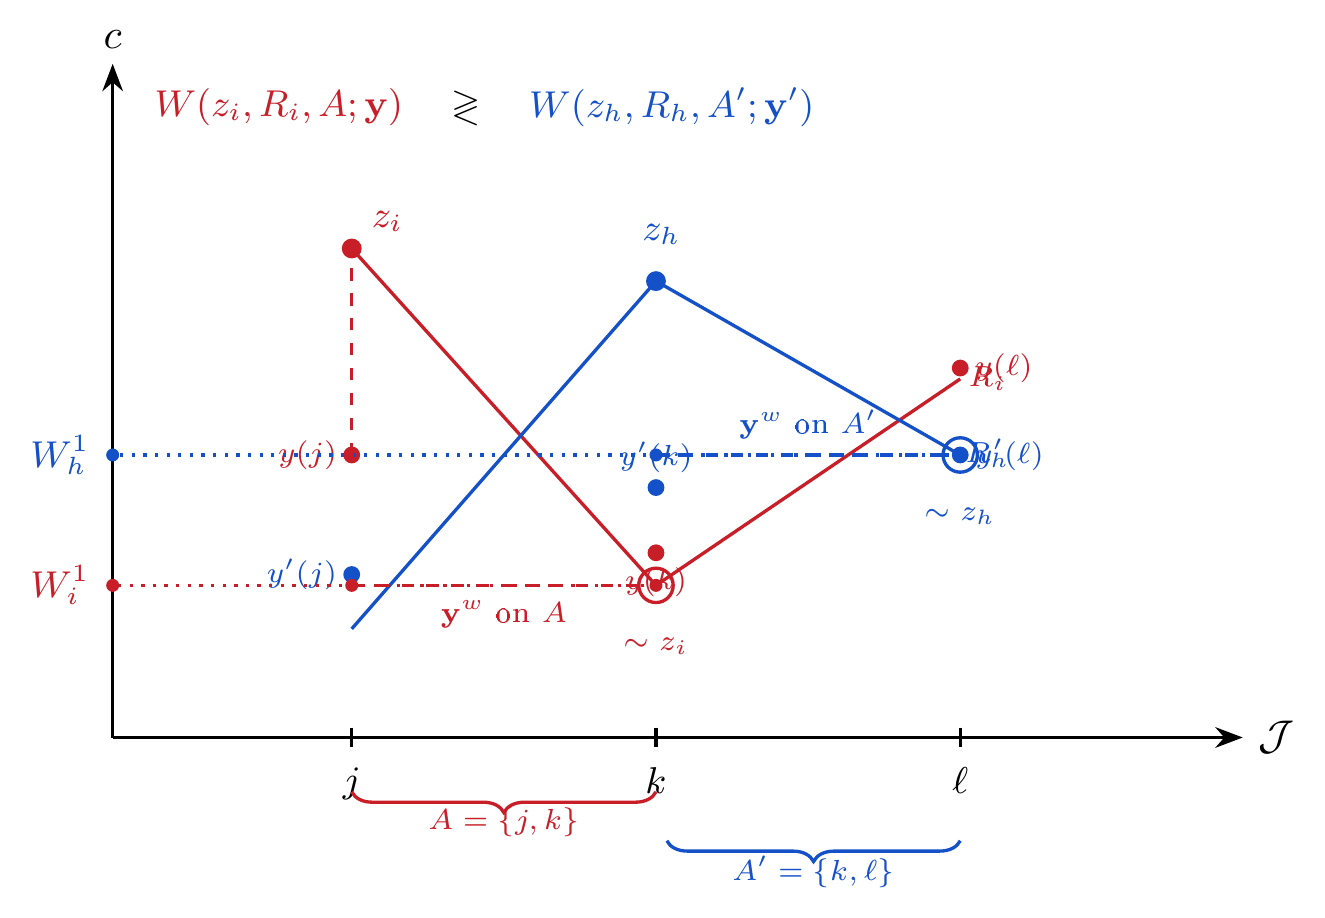
\includegraphics[height=0.57\textheight,width=\textwidth,keepaspectratio]{theory_w1.png}
\end{center}
{\footnotesize Own-set equal-consumption equivalents: each individual gets a common consumption on every job in their own ability set; the level at which the preferred job is indifferent to the attained bundle is their money metric, comparable across individuals. Adapted from Haydar and Maniquet (2026), work in progress.\par}
\cornerlinks{\golink{b:attderiv}{ATT derivation} \golink{b:eaderiv}{EA derivation}}
\note{Estimated utility is not an interpersonal welfare index: preferences
differ, so the same utility number means different things for different people.
Each situation is translated into euros through an indifference condition with
an explicit reference, and the choice of reference is the welfare question.

Both money metrics descend from this construction in the companion theory paper.
Each individual is evaluated with their own preferences and their own set of
jobs. Give every job in that set the same consumption; the consumption at which
the preferred job is exactly as good as the attained bundle is their money
metric. The next two slides take the construction to the data in two ways.}
\end{frame}

% ==================================================================== EA
\begin{frame}
\frametitle{Ex-ante prospect welfare}
\hypertarget{main:ea}{}
\slideeq{$\displaystyle\begin{gathered}
  J_i=\int e^{L_i(j)}\Big(\tfrac{C_i(j)}{\lambda_c}\Big)^{\beta_c}\,\widehat g_i(j)\,d\nu(j),
  \qquad
  H_i=\int e^{L_i(j)}\,\widehat g_i(j)\,d\nu(j),
  \\[0.35em]
  M^{\mathrm{EA}}_i=\lambda_c\exp\!\Big\{\tfrac{\log J_i-\log H_i}{\beta_c}\Big\}
  \end{gathered}$}
\begin{columns}[T,onlytextwidth]
\column{0.31\textwidth}\centering
$J_i$\\ {\footnotesize the actual prospect}
\column{0.31\textwidth}\centering
$H_i$\\ {\footnotesize same jobs, equal pay}
\column{0.31\textwidth}\centering
$M^{\mathrm{EA}}_i$\\ {\footnotesize flat-consumption equivalent}
\end{columns}
\vfill
\cornerlinks{\golink{b:eaderiv}{derivation} \golink{b:eavalid}{numerical validation}}
\note{In words: EA is the constant monthly consumption at which a prospect with
the household's own jobs and availability, but equal pay everywhere, is worth
exactly as much as the prospect it actually faces.

Every job enters J weighted by how available it is and how much it is valued; H
keeps the same jobs, availability and preferences with pay differences removed.
Opportunities enter welfare directly: access moves which jobs carry weight;
earning opportunities move what they pay.

I show this perspective first because this talk is about opportunities; that is
an order of presentation, not a ranking. The measure treats taste-shock variety
as part of what makes a rich prospect valuable, which is a normative position.}
\end{frame}

% ==================================================================== ATT
\begin{frame}
\frametitle{Attained-bundle welfare}
\hypertarget{main:att}{}
\slideeq{$\displaystyle M^{\mathrm{att}}_i=C^{\mathrm{obs}}_i\exp\!\left\{\frac{L_i(j^{\mathrm{obs}}_i)-L_i(o)}{\beta_c}\right\}$}
\begin{columns}[T,onlytextwidth]
\column{0.46\textwidth}\centering
$o$\\ {\footnotesize non-employment, reachable by all}
\column{0.46\textwidth}\centering
$j^{\mathrm{obs}}_i$\\ {\footnotesize the only route for opportunities}
\end{columns}
\vfill
\cornerlinks{\golink{b:attderiv}{derivation}}
\note{In words: ATT is observed consumption, adjusted by the leisure the job
costs relative to not working, converted at the rate one over the consumption
weight.

The reference is non-employment, which every household can reach. On the
current empirical domain the equal-consumption reference job is non-employment
for every household, so the measure coincides with the staying-home equivalent;
that is a property of this specification, not a theorem. Opportunities matter
only through which job is attained and what it pays.

The two measures answer different welfare questions: one values the prospect,
the other the attained outcome. Neither corrects the other.}
\end{frame}

% ==================================================================== Shapley
\begin{frame}
\frametitle{Inequality and Shapley decomposition}
\hypertarget{main:shapley}{}
\vfill
\begin{columns}[T,onlytextwidth]
\column{0.23\textwidth}\centering
\textcolor{chpref}{\textbf{P}}\\ {\footnotesize preferences: age, children}
\column{0.23\textwidth}\centering
\textcolor{chacc}{\textbf{A}}\\ {\footnotesize local unemployment exposure, region, urban or rural location, year}
\column{0.23\textwidth}\centering
\textcolor{chearn}{\textbf{B}}\\ {\footnotesize wage-offer location}
\column{0.23\textwidth}\centering
\textcolor{chneeds}{\textbf{held fixed}}\\ {\footnotesize household resources, needs and composition}
\end{columns}
\slideeq{$\displaystyle\phi^p_k=\sum_{S\subseteq\{P,A,B\}\setminus\{k\}}\frac{|S|!\,(3-|S|-1)!}{3!}\Big[v^p(S\cup\{k\})-v^p(S)\Big]$}
\begin{center}
$v^p(S)=I^p(\varnothing)-I^p(S)$ \qquad $I^p$: household-weighted Gini of $M^p$
\end{center}
\vfill
\cornerlinks{\golink{b:shapley}{Shapley vs one-factor} \golink{b:eagini}{full tables}}
\note{In words: a channel's Shapley contribution is its marginal effect on
inequality, averaged over every order in which the three equalisations can be
introduced; the three contributions add up exactly to the total change.

P equalises age profiles and the child-related shifter. A equalises local
access: local unemployment exposure, region, urban or rural location, and year;
it is local access, not total opportunity. B equalises the systematic wage-offer
location, not wage dispersion. Household resources, needs and composition are
held fixed in every coalition.

Each coalition is a full structural counterfactual: coefficients never change,
welfare is recomputed for every household under each perspective, and inequality
is measured again. Contributions are signed.}
\end{frame}

% ==================================================================== how much
\begin{frame}
\frametitle{How much is associated with opportunities?}
\hypertarget{main:howmuch}{}
\vspace{0.2em}
\begin{center}
\renewcommand{\arraystretch}{1.05}
\begin{tabular}{>{\raggedright\arraybackslash}p{0.34\textwidth}>{\centering\arraybackslash}p{0.22\textwidth}>{\centering\arraybackslash}p{0.22\textwidth}}
 & \textbf{Single adults} & \textbf{Couples} \\[0.2em]
\textcolor{chacc}{\textbf{Ex-ante prospect}}\newline{\small equivalised} & {\huge \VEASingOppEq\%} & {\huge \VEACoupOppEq\%} \\
 & {\color{gray}\scriptsize raw \VEASingOppRaw\%} & {\color{gray}\scriptsize raw \VEACoupOppRaw\%} \\[0.5em]
\textcolor{chearn}{\textbf{Attained bundle}}\newline{\small equivalised} & {\huge \VAttSingOppEq\%} & {\huge \VAttCoupOppEq\%} \\
 & {\color{gray}\scriptsize raw \VAttSingOppRaw\%} & {\color{gray}\scriptsize raw \VAttCoupOppRaw\%} \\
\end{tabular}
\end{center}
\vfill
\begin{center}
\textbf{A + B as \% of the relevant baseline Gini}
\end{center}
{\scriptsize\color{gray} Household resources, needs and composition held fixed \quad$\cdot$\quad A is the currently estimated local-access channel\par}
\cornerlinks{\golink{b:eagini}{EA decomposition} \golink{b:attgini}{ATT decomposition} \golink{b:equiv}{equivalisation} \golink{b:central}{figure}}
\note{This is the first result. Each number is local access plus earning
opportunities, the A plus B part of the restricted game, as a percentage of that
perspective's own baseline Gini, on the equivalised scale.

When welfare values the whole prospect, the two opportunity channels are
associated with \VEASingOppEq{} per cent of baseline inequality for single adults
and \VEACoupOppEq{} per cent for couples. When welfare values the attained bundle
they are associated with \VAttSingOppEq{} and \VAttCoupOppEq{} per cent.

The small grey numbers are the raw household scale, for reference only.
Household resources, needs and composition are held fixed, and A is the local
access channel as currently estimated. Prospects versus attained outcomes: the
two perspectives answer different welfare questions, and neither is designated
primary. None of these is a causal share.}
\end{frame}

% ==================================================================== which channel
\begin{frame}
\frametitle{Which opportunity channel matters?}
\hypertarget{main:channel}{}
\vfill
\begin{columns}[T,onlytextwidth]
\column{0.46\textwidth}
\centering
\textbf{Single adults}\\[0.6em]
{\small\textcolor{chacc}{access}}\\
{\Huge \VChEASingAEq\%}\\[0.5em]
{\small\textcolor{chearn}{earning opportunities}}\\
{\Huge \VChEASingBEq\%}\\[0.5em]
{\small A + B $=$ \VEASingOppEq\%}
\column{0.46\textwidth}
\centering
\textbf{Couples}\\[0.6em]
{\small\textcolor{chacc}{access}}\\
{\Huge \VChEACoupAEq\%}\\[0.5em]
{\small\textcolor{chearn}{earning opportunities}}\\
{\Huge \VChEACoupBEq\%}\\[0.5em]
{\small A + B $=$ \VEACoupOppEq\%}
\end{columns}
\vfill
\begin{center}
{\small ex-ante prospect, equivalised: \% of baseline Gini}\\[0.3em]
single adults: access $>$ earnings \qquad couples: earnings $>$ access, close\\[0.3em]
{\small attained bundle: earnings $>$ access for both populations}
\end{center}
\cornerlinks{\golink{b:eapct}{EA channels} \golink{b:attpct}{ATT channels}}
\note{Now split the ex-ante number into its two channels, each as a percentage
of the baseline Gini on the equivalised scale.

For single adults, local access is the larger channel, about three times earning
opportunities. For couples, earning opportunities are larger than access, but
the two are close on this scale.

Under the attained-bundle perspective the ordering is the other way for single
adults: earning opportunities are larger than access for both populations. The
full tables, with Gini points and the raw scale, are one click away. These are
accounting shares within a restricted game, not causal shares.}
\end{frame}

% ==================================================================== 100 per cent
\begin{frame}
\frametitle{Where does baseline inequality go?}
\hypertarget{main:hundred}{}
{\scriptsize\color{gray} shares of baseline Gini \ $\cdot$\ ex-ante prospect, equivalised \ $\cdot$\ current restricted P/A/B game \ $\cdot$\ A $=$ current local-access channel\par}
\vspace{-0.6em}
\begin{center}\small
\renewcommand{\arraystretch}{1.0}
\begin{tabular}{>{\raggedright\arraybackslash}p{0.62\textwidth}rr}
\toprule
 & \textbf{Single adults} & \textbf{Couples} \\
\midrule
\textcolor{chpref}{Preferences} \quad $\phi_P/I_0$ & \VHundredSingP\% & \VHundredCoupP\% \\
\textcolor{chacc}{Local access} \quad $\phi_A/I_0$ & \VHundredSingA\% & \VHundredCoupA\% \\
\textcolor{chearn}{Earning opportunities} \quad $\phi_B/I_0$ & \VHundredSingB\% & \VHundredCoupB\% \\
\textbf{Not allocated by this exercise} \quad $1-(\phi_P+\phi_A+\phi_B)/I_0$ & \VHundredSingRest\% & \VHundredCoupRest\% \\
\midrule
Total & \VHundredSingTotal\% & \VHundredCoupTotal\% \\
\bottomrule
\end{tabular}
\end{center}
\vfill
\vspace{-0.8em}
{\scriptsize Couples: A + B alone $=$ \VHundredCoupAB\%; P + A + B $=$ \VHundredCoupExplained\% because the preference contribution is negative (\VHundredCoupP\%).\par}
\vspace{0.15em}
{\scriptsize Not allocated is not a channel: it holds household resources, needs and composition fixed, retains sex-specific preference and opportunity blocks, and excludes wage-draw luck and the common offer spread, which exceed the location differences equalised.\par}
\vspace{0.1em}
{\tiny\color{gray} one decimal; the not-allocated row closes each column to the total\par}
\vspace{1.0em}
\cornerlinks{\golink{b:eapct}{channels in Gini points} \golink{b:residual}{not allocated}}
\note{Here is the same ex-ante decomposition, laid out so that it visibly sums to
the whole baseline Gini, on the equivalised scale.

Under the current restricted ex-ante decomposition, labour-market opportunities
are associated with about \VHundredSingAB{} per cent of baseline welfare
inequality for single adults and about \VHundredCoupAB{} per cent for couples.

For couples the preference contribution is negative, so preferences plus access
plus earnings is smaller than access plus earnings alone; the table shows the
negative row rather than hiding it.

The last row is not a channel and it is not needs explaining the rest. It is
what this exercise does not allocate: household resources, needs and
composition are held fixed, sex-specific blocks are kept, and the wage-draw
luck and common offer spread are not equalised; those are larger than the
location differences that the access and earning operators remove. None of
these shares is causal.}
\end{frame}

% ==================================================================== not claimed
\begin{frame}
\frametitle{What is not claimed}
\hypertarget{main:limits}{}
\vfill
\begin{columns}[T,onlytextwidth]
\column{0.46\textwidth}
\centering
\textbf{Scope}\\[0.6em]
{\small Household resources, needs and composition held fixed}\\[0.5em]
{\small Access: local access, not total opportunity}\\[0.5em]
{\small Preliminary decomposition}
\column{0.46\textwidth}
\centering
\textbf{Not claimed}\\[0.6em]
{\small Not causal}\\[0.5em]
{\small No parameter uncertainty yet}\\[0.5em]
{\small Preferences are not responsibility}\\[0.5em]
{\small Neither perspective is designated primary}
\end{columns}
\vfill
\begin{center}
{\small prospects versus attained outcomes: two different welfare questions}
\end{center}
\vfill
\cornerlinks{\golink{b:residual}{not allocated} \golink{b:robust}{robustness}}
\note{All the boundaries in one place.

The decomposition is preliminary: a restricted structural accounting exercise,
and the attained-bundle counterfactual integration is still being validated,
with short hours sparsely covered. Nothing is causal: separation rests on
maintained functional-form and exclusion restrictions. Parameter uncertainty has
not been propagated through either decomposition. The preference channel is not
a responsibility channel; deciding what people should be held responsible for is
a normative step this paper does not take. Household resources, needs and
composition are held fixed, and access is local access, not total opportunity.
The two welfare perspectives answer different questions, and choosing between
them is a normative decision not made here.}
\end{frame}

% ==================================================================== conclusion
\begin{frame}
\frametitle{Conclusion}
\hypertarget{main:conclusion}{}
\vfill
\begin{enumerate}\itemsep0.9em
  \item Choices reflect opportunities, not preferences alone.
  \item Prospects: access leads for single adults.\quad Attained outcomes: earnings lead.\quad Couples: no reversal.
  \item Restricted P/A/B: a bounded part of well-being inequality; preference sign not robust.
\end{enumerate}
\vfill
\begin{center}
{\small next: resources and needs as a fourth channel \quad$\cdot$\quad parameter uncertainty \quad$\cdot$\quad validation}
\end{center}
\vfill
\cornerlinks{\golink{main:limits}{limitations} \golink{b:residual}{next steps} \golink{appmap}{appendix map}}
\note{To close, the three answers.

First, observed choices carry information about opportunities: a model that
gives everyone the same jobs fits worse on the same households.

Second, the importance assigned to different labour-market inequalities depends
on whether welfare evaluates the opportunity prospect or the realised outcome.
Access leads for single adults when we value the prospect; earning
opportunities lead when we value the attained bundle; couples do not reverse.

Third, within the restricted decomposition, local access and earning
opportunities are a bounded part of well-being inequality, and the preference
contribution is not sign-robust to equivalisation.

Next steps: household resources, needs and composition as a fourth channel;
propagating parameter uncertainty; completing validation of the attained-bundle
integration. Neither perspective is designated primary. Thank you.}
\end{frame}

% ============================================================ BACKUP
\appendix

% ==================================================================== map
\begin{frame}
\frametitle{Appendix map}
\hypertarget{appmap}{}
\vfill
\begin{center}\scriptsize
\renewcommand{\arraystretch}{1.5}
\setlength{\tabcolsep}{4pt}
\begin{tabular}{>{\bfseries}l llll}
Model & \maplink{b:utility}{Utility specification} & \maplink{b:density}{Opportunity density} & \maplink{b:likelihood}{Likelihood} & \maplink{b:ident}{Identification} \\
Estimation & \maplink{b:prefs}{Preferences} & \maplink{b:access}{Employment access} & \maplink{b:hours}{Hours and occupation} & \maplink{b:wage}{Wage offers} \\
 & \maplink{b:benchmarks}{Common opportunities} & \maplink{b:inference}{Inference} & & \\
Fit & \maplink{b:extensive}{Extensive margin} & \maplink{b:margins}{Fit by margin} & \maplink{b:hours37}{Thirty-seven-hour point} & \maplink{b:matched}{Matched households} \\
 & \maplink{b:mrs}{Marginal rate of substitution} & & & \\
Welfare & \maplink{b:attderiv}{ATT derivation} & \maplink{b:eaderiv}{EA derivation} & \maplink{b:eavalid}{EA validation} & \maplink{b:equiv}{Equivalisation} \\
Decomposition & \maplink{b:central}{Central figure} & \maplink{b:eagini}{EA Gini points} & \maplink{b:attgini}{ATT Gini points} & \maplink{b:eapct}{EA channel shares} \\
 & \maplink{b:attpct}{ATT channel shares} & \maplink{b:explained}{Composition within P/A/B} & \maplink{b:shapley}{Shapley vs one-factor} & \maplink{b:residual}{Not allocated} \\
 & \maplink{b:robust}{Robustness} & & & \\
Data & \maplink{b:sample}{Sample selection} & \maplink{b:pricing}{EUROMOD pricing} & \maplink{b:numerics}{Numerical design} & \\
\end{tabular}
\end{center}
\vfill
\cornerlinks{\hyperlink{main:conclusion}{\beamerreturnbutton{Back}}}
\note{The appendix map. Every entry is a link; every backup slide has a Back
button to the main slide it supports and a button back to this map.}
\end{frame}

% ==================================================================== MODEL
\begin{frame}
\frametitle{Backup: utility specification}
\hypertarget{b:utility}{}
\vfill
\backupeq{$\displaystyle v_i(j)=L_i(j)+\beta_c\log\!\Big(\frac{C_i(j)}{\lambda_c}\Big),\qquad
L_i(j)=\beta^g_\ell(\mathbf x_i)\,\mathcal B\big(\tilde\ell_i(j);\theta^g_\ell\big)$}
\backupeq{$\displaystyle \tilde\ell_i(j)=\frac{\VTimeEndow-h}{\VLeisureScale},\qquad \mathcal B(z;\theta)=\frac{z^\theta-1}{\theta}$}
\vfill
\begin{columns}[T,onlytextwidth]
\column{0.31\textwidth}\centering
$\beta^g_\ell(\mathbf x_i)$\\ {\footnotesize intercept, centred age and its square (units of \VAgeScale{} years)}
\column{0.31\textwidth}\centering
$k_i$\\ {\footnotesize children under \VChildCutoff, women only}
\column{0.31\textwidth}\centering
couples\\ {\footnotesize sum of the two spouses' leisure terms}
\end{columns}
\vfill
\backnav{main:jobs}
\note{The full systematic utility. Leisure is weekly time left from a maintained
endowment, rescaled, and passed through a Box-Cox transform with a group-specific
curvature. The leisure weight varies with centred age and, for women, with the
number of children; that child term is a reduced-form time-constraint shifter,
not pure taste. The consumption weight is estimated. The shock is extreme value
with unit scale.}
\end{frame}

\begin{frame}
\frametitle{Backup: opportunity density}
\hypertarget{b:density}{}
\vfill
\backupeq{$\displaystyle g_i(j)=g^{E}_i\cdot\Big(g^{H}_i(h)\;g^{\mathrm{Occ}}_i(k)\;g^{W}_i(w\mid k)\Big)^{E_i(j)}$}
\vfill
\begin{columns}[T,onlytextwidth]
\column{0.23\textwidth}\centering
\textcolor{chacc}{\textbf{access}}\\ {\footnotesize $g^E_i$: local unemployment exposure, region, urban or rural location, year}
\column{0.23\textwidth}\centering
\textbf{hours}\\ {\footnotesize $g^H_i$: elevated bands over a residual set}
\column{0.23\textwidth}\centering
\textbf{occupation}\\ {\footnotesize $g^{\mathrm{Occ}}_i$: sex-specific group masses}
\column{0.23\textwidth}\centering
\textcolor{chearn}{\textbf{wage offers}}\\ {\footnotesize $g^W_i$: log-normal, truncated to $[\VWageLo,\VWageHi]$}
\end{columns}
\vfill
\begin{center}
{\small wage-offer location $\mu_i(k)$: education, potential experience and its square, occupation}
\end{center}
\vfill
\backnav{main:opp}
\note{The opportunity density factorises into access, switched on for employment,
and three blocks for the employed part: hours, occupation and wage offers. The
unemployment exposure enters access scaled by \VGsurScale. The wage location
depends on education, potential experience in units of \VExpScale{} years and
occupation, with a common dispersion. The hours density is a density elevation
over intervals, not an atom at a particular hour.}
\end{frame}

\begin{frame}
\frametitle{Backup: sampled-alternative likelihood}
\hypertarget{b:likelihood}{}
\vfill
\backupeq{$\displaystyle V_{ij}=v_i(j)+\log g_i(j)-\log q_{ij}$}
\backupeq{$\displaystyle \Pr\!\big(y\mid\mathcal C_i\big)=\frac{n_y\exp V_{iy}}{\sum_{s\in\mathcal C_i}\exp V_{is}}$}
\vfill
\begin{columns}[T,onlytextwidth]
\column{0.31\textwidth}\centering
$q_{ij}$\\ {\footnotesize proposal density, fitted out of fold}
\column{0.31\textwidth}\centering
$\mathcal C_i$\\ {\footnotesize observed job and \VNDraws{} draws: \VNAltRows{} rows}
\column{0.31\textwidth}\centering
$n_y$\\ {\footnotesize multiplicity of a repeated draw}
\end{columns}
\vfill
\backnav{main:opp}
\note{The choice set is a continuum, so the likelihood is evaluated over sampled
alternatives drawn from a proposal density and corrected by it. The proposal is a
computational device: fitted out of fold so a household's own outcome never
enters the proposal used to score it, and it enters no welfare measure. For
couples the proposal draws the joint participation regime first.}
\end{frame}

\begin{frame}
\frametitle{Backup: identification}
\hypertarget{b:ident}{}
\vfill
\begin{columns}[T,onlytextwidth]
\column{0.31\textwidth}\centering
\textbf{Functional form}\\[0.4em]
{\footnotesize smooth preferences in hours; banded hours opportunities}
\column{0.31\textwidth}\centering
\textbf{Exclusion}\\[0.4em]
{\footnotesize local unemployment exposure and geography shift access, not utility}
\column{0.31\textwidth}\centering
\textbf{Independence}\\[0.4em]
{\footnotesize wage offers independent of hours, given occupation}
\end{columns}
\vfill
\begin{center}
{\small maintained, not tested \quad$\cdot$\quad not a causal design}
\end{center}
\vfill
\backnav{main:est}
\note{Choices alone do not separate a taste for leisure from a scarcity of jobs at
that number of hours. Three restrictions do the work: a spike at a band of hours
is read as availability rather than a kink in tastes; excluded shifters enter
availability and not preferences; and wage offers are independent of hours given
occupation. These are the restrictions of the latent-jobs literature, maintained
here rather than tested. No causal effect of geography is claimed.}
\end{frame}

% ==================================================================== ESTIMATION
\begin{frame}
\frametitle{Backup: preference parameters}
\hypertarget{b:prefs}{}
\vfill
\begin{center}\scriptsize
\renewcommand{\arraystretch}{1.3}
\begin{tabular}{lcccc}
\toprule
 & Single men & Single women & Couple men & Couple women \\
\midrule
leisure weight, intercept & \VCoefSingBetaZeroLSm{} \se{\VCoefSingBetaZeroLSmSE} & \VCoefSingBetaZeroLSf{} \se{\VCoefSingBetaZeroLSfSE} & \VCoefCoupBetaZeroLM{} \se{\VCoefCoupBetaZeroLMSE} & \VCoefCoupBetaZeroLF{} \se{\VCoefCoupBetaZeroLFSE} \\
leisure weight, age & \VCoefSingBetaLAgeSm{} \se{\VCoefSingBetaLAgeSmSE} & \VCoefSingBetaLAgeSf{} \se{\VCoefSingBetaLAgeSfSE} & \VCoefCoupBetaLAgeM{} \se{\VCoefCoupBetaLAgeMSE} & \VCoefCoupBetaLAgeF{} \se{\VCoefCoupBetaLAgeFSE} \\
leisure weight, age squared & \VCoefSingBetaLTwoAgeSm{} \se{\VCoefSingBetaLTwoAgeSmSE} & \VCoefSingBetaLTwoAgeSf{} \se{\VCoefSingBetaLTwoAgeSfSE} & \VCoefCoupBetaLTwoAgeM{} \se{\VCoefCoupBetaLTwoAgeMSE} & \VCoefCoupBetaLTwoAgeF{} \se{\VCoefCoupBetaLTwoAgeFSE} \\
leisure weight, children & --- & \VCoefSingBetaLNkidsSf{} \se{\VCoefSingBetaLNkidsSfSE} & --- & \VCoefCoupBetaLNkidsF{} \se{\VCoefCoupBetaLNkidsFSE} \\
leisure curvature $\theta_\ell$ & \VCoefSingThetaLSm{} \se{\VCoefSingThetaLSmSE} & \VCoefSingThetaLSf{} \se{\VCoefSingThetaLSfSE} & \VCoefCoupThetaLM{} \se{\VCoefCoupThetaLMSE} & \VCoefCoupThetaLF{} \se{\VCoefCoupThetaLFSE} \\
consumption weight $\beta_c$ & \multicolumn{2}{c}{\VCoefSingBetaC{} \se{\VCoefSingBetaCSE}} & \multicolumn{2}{c}{\VCoefCoupBetaC{} \se{\VCoefCoupBetaCSE}} \\
\bottomrule
\end{tabular}
\end{center}
\vfill
{\footnotesize cluster-robust standard errors; the male children term in couples is structurally zero}
\backnav{main:sel}
\note{The preference block. The consumption weight is common within each
population. One single-adult coordinate, the female age-square term, sits at a
box endpoint, so its standard error is not reported and it is excluded from the
interior curvature. Levels are not comparable across the two separately
estimated models.}
\end{frame}

\begin{frame}
\frametitle{Backup: employment-access parameters}
\hypertarget{b:access}{}
\vfill
\begin{center}\scriptsize
\renewcommand{\arraystretch}{1.12}
\begin{tabular}{lcc}
\toprule
 & Singles & Couples \\
\midrule
employment constant & \VCoefSingBetaE{} \se{\VCoefSingBetaESE} & men \VCoefCoupBetaEM{} \se{\VCoefCoupBetaEMSE}; women \VCoefCoupBetaEF{} \se{\VCoefCoupBetaEFSE} \\
local unemployment exposure & \VCoefSingBetaEGsur{} \se{\VCoefSingBetaEGsurSE} & \VCoefCoupBetaEGsur{} \se{\VCoefCoupBetaEGsurSE} \\
densely populated & \VCoefSingBetaEDrgur{} \se{\VCoefSingBetaEDrgurSE} & \VCoefCoupBetaEDrgur{} \se{\VCoefCoupBetaEDrgurSE} \\
intermediate density & \VCoefSingBetaEDrgmd{} \se{\VCoefSingBetaEDrgmdSE} & \VCoefCoupBetaEDrgmd{} \se{\VCoefCoupBetaEDrgmdSE} \\
\VCoefSingBetaETwoDrgnLabel & \VCoefSingBetaETwoDrgn{} \se{\VCoefSingBetaETwoDrgnSE} & \VCoefCoupBetaETwoDrgn{} \se{\VCoefCoupBetaETwoDrgnSE} \\
\VCoefSingBetaEThreeDrgnLabel & \VCoefSingBetaEThreeDrgn{} \se{\VCoefSingBetaEThreeDrgnSE} & \VCoefCoupBetaEThreeDrgn{} \se{\VCoefCoupBetaEThreeDrgnSE} \\
\VCoefSingBetaEFourDrgnLabel & \VCoefSingBetaEFourDrgn{} \se{\VCoefSingBetaEFourDrgnSE} & \VCoefCoupBetaEFourDrgn{} \se{\VCoefCoupBetaEFourDrgnSE} \\
\VCoefSingBetaEFiveDrgnLabel & \VCoefSingBetaEFiveDrgn{} \se{\VCoefSingBetaEFiveDrgnSE} & \VCoefCoupBetaEFiveDrgn{} \se{\VCoefCoupBetaEFiveDrgnSE} \\
\VCoefSingBetaESixDrgnLabel & \VCoefSingBetaESixDrgn{} \se{\VCoefSingBetaESixDrgnSE} & \VCoefCoupBetaESixDrgn{} \se{\VCoefCoupBetaESixDrgnSE} \\
\VCoefSingBetaESevenDrgnLabel & \VCoefSingBetaESevenDrgn{} \se{\VCoefSingBetaESevenDrgnSE} & \VCoefCoupBetaESevenDrgn{} \se{\VCoefCoupBetaESevenDrgnSE} \\
\VCoefSingBetaEEightDrgnLabel & \VCoefSingBetaEEightDrgn{} \se{\VCoefSingBetaEEightDrgnSE} & \VCoefCoupBetaEEightDrgn{} \se{\VCoefCoupBetaEEightDrgnSE} \\
\bottomrule
\end{tabular}
\end{center}
\vfill
{\footnotesize references: the first region and thinly populated areas; couples share the shifters across spouses}
\backnav{main:sel}
\note{The employment-access block. The employment index multiplies the working
indicator. Local unemployment exposure lowers employment opportunity mass in both
populations. Regional and urbanisation indicators shift access conditional on the
exclusion restriction; they are not causal effects of geography.}
\end{frame}

\begin{frame}
\frametitle{Backup: hours and occupation opportunities}
\hypertarget{b:hours}{}
\vfill
\begin{center}\scriptsize
\textbf{Hours bands}\\[0.3em]
\renewcommand{\arraystretch}{1.05}
\begin{tabular}{lccc}
\toprule
 & Singles & Couple men & Couple women \\
\midrule
part-time lower & \VCoefSingBetaHOnePt & \VCoefCoupBetaHOnePtM & \VCoefCoupBetaHOnePtF \\
part-time upper & \VCoefSingBetaHTwoPt & \VCoefCoupBetaHTwoPtM & \VCoefCoupBetaHTwoPtF \\
narrow full-time & \VCoefSingBetaHThreeFiveF & \VCoefCoupBetaHThreeFiveFM & \VCoefCoupBetaHThreeFiveFF \\
full-time upper & \VCoefSingBetaHFt & \VCoefCoupBetaHFtM & \VCoefCoupBetaHFtF \\
long hours & \VCoefSingBetaHLh & \VCoefCoupBetaHLhM & \VCoefCoupBetaHLhF \\
\bottomrule
\end{tabular}\\[0.6em]
\textbf{Occupation masses}\\[0.3em]
\renewcommand{\arraystretch}{1.05}
\begin{tabular}{lcccc}
\toprule
 & \multicolumn{2}{c}{Singles} & \multicolumn{2}{c}{Couples} \\
 & men & women & men & women \\
\midrule
\VCoefSingBetaOccTwoMLabel & \VCoefSingBetaOccTwoM & \VCoefSingBetaOccTwoF & \VCoefCoupBetaOccTwoM & \VCoefCoupBetaOccTwoF \\
\VCoefSingBetaOccThreeMLabel & \VCoefSingBetaOccThreeM & \VCoefSingBetaOccThreeF & \VCoefCoupBetaOccThreeM & \VCoefCoupBetaOccThreeF \\
\VCoefSingBetaOccFourMLabel & \VCoefSingBetaOccFourM & \VCoefSingBetaOccFourF & \VCoefCoupBetaOccFourM & \VCoefCoupBetaOccFourF \\
\bottomrule
\end{tabular}
\end{center}
\vfill
{\footnotesize estimates only; standard errors in the paper. References: the residual hours set and the craft and elementary occupation group}
\backnav{main:sel}
\note{Hours opportunities are elevated densities over five bands relative to a
residual set; hours coefficients are common across single men and women and
spouse-specific for couples. Occupation masses are sex-specific, relative to the
craft, agricultural, operator and elementary group. Standard errors for these
blocks are in the paper's tables.}
\end{frame}

\begin{frame}
\frametitle{Backup: wage-offer equation}
\hypertarget{b:wage}{}
\vfill
\begin{center}\scriptsize
\renewcommand{\arraystretch}{1.2}
\begin{tabular}{lcc}
\toprule
 & Singles & Couples \\
\midrule
intercept & \VCoefSingBetaZeroW{} \se{\VCoefSingBetaZeroWSE} & \VCoefCoupBetaZeroW{} \se{\VCoefCoupBetaZeroWSE} \\
low education & \VCoefSingBetaWEducL{} \se{\VCoefSingBetaWEducLSE} & \VCoefCoupBetaWEducL{} \se{\VCoefCoupBetaWEducLSE} \\
high education & \VCoefSingBetaWEducH{} \se{\VCoefSingBetaWEducHSE} & \VCoefCoupBetaWEducH{} \se{\VCoefCoupBetaWEducHSE} \\
potential experience & \VCoefSingBetaWPexp{} \se{\VCoefSingBetaWPexpSE} & \VCoefCoupBetaWPexp{} \se{\VCoefCoupBetaWPexpSE} \\
experience squared & \VCoefSingBetaWTwoPexp{} \se{\VCoefSingBetaWTwoPexpSE} & \VCoefCoupBetaWTwoPexp{} \se{\VCoefCoupBetaWTwoPexpSE} \\
\VCoefSingDeltaOccTwoLabel & \VCoefSingDeltaOccTwo{} \se{\VCoefSingDeltaOccTwoSE} & \VCoefCoupDeltaOccTwo{} \se{\VCoefCoupDeltaOccTwoSE} \\
\VCoefSingDeltaOccThreeLabel & \VCoefSingDeltaOccThree{} \se{\VCoefSingDeltaOccThreeSE} & \VCoefCoupDeltaOccThree{} \se{\VCoefCoupDeltaOccThreeSE} \\
\VCoefSingDeltaOccFourLabel & \VCoefSingDeltaOccFour{} \se{\VCoefSingDeltaOccFourSE} & \VCoefCoupDeltaOccFour{} \se{\VCoefCoupDeltaOccFourSE} \\
log-wage dispersion $\sigma$ & \VCoefSingSigma{} \se{\VCoefSingSigmaSE} & \VCoefCoupSigma{} \se{\VCoefCoupSigmaSE} \\
\bottomrule
\end{tabular}
\end{center}
\vfill
{\footnotesize medium education is the reference; experience in units of \VExpScale{} years}
\backnav{main:sel}
\note{The wage-offer equation. The offered log wage is normal with this location
and a common dispersion, truncated to the wage support and renormalised. The
singles and couples models are estimated separately, so the two experience
profiles are not restricted to agree and their difference is not a test.}
\end{frame}

\begin{frame}
\frametitle{Backup: common versus household-specific opportunities}
\hypertarget{b:benchmarks}{}
\vfill
\begin{center}\small
\renewcommand{\arraystretch}{1.35}
\begin{tabular}{>{\raggedright\arraybackslash}p{0.44\textwidth}ccc}
\toprule
Single adults & free coordinates & criterion & population fit \\
\midrule
household-specific opportunities & \VKFreeSingles{} & \VNegllSingles{} & \VMaeSingles{} \\
common opportunity distribution & \VKFreeRumA{} & \VNegllRumA{} & \VMaeRumA{} \\
common shape; employment and hours in utility & \VKFreeRumB{} & \VNegllRumB{} & \VMaeRumB{} \\
\bottomrule
\end{tabular}
\end{center}
\vfill
{\footnotesize same households, sampled alternatives and criterion; not converted into a formal test}
\backnav{main:est}
\note{The two re-estimated common-opportunity benchmarks restrict the opportunity
block and re-estimate everything else. Both are worse on the same criterion, and
population fit worsens where the opportunity block does its work. A better
criterion does not by itself establish that a mechanism has been identified.}
\end{frame}

\begin{frame}
\frametitle{Backup: curvature and inference}
\hypertarget{b:inference}{}
\vfill
\begin{columns}[T,onlytextwidth]
\column{0.46\textwidth}
\centering
\textbf{Single adults}\\[0.5em]
{\small free coordinates \VKFreeSingles{}, interior \VKIntSingles{}}\\
{\small criterion \VNegllSingles{}}\\
{\small smallest Hessian eigenvalue \VMinEigSingles{}}
\column{0.46\textwidth}
\centering
\textbf{Couples}\\[0.5em]
{\small free coordinates \VKFreeCouples{}, interior \VKIntCouples{}}\\
{\small criterion \VNegllCouples{}}\\
{\small smallest Hessian eigenvalue \VMinEigCouples{}}
\end{columns}
\vfill
\begin{center}
{\small cluster-robust standard errors on the household \quad$\cdot$\quad eigenvalues on the interior block}
\end{center}
\vfill
\backnav{main:sel}
\note{Curvature and inference. The exact Hessian on the interior block is
positive definite for both models. Several terminal paths from different starts
agree to numerical precision; that supports a stable local solution from the
starts tested, not global uniqueness. One single-adult coordinate at a box
endpoint is handled under the active-set convention.}
\end{frame}

% ==================================================================== FIT
\begin{frame}
\frametitle{Backup: extensive-margin fit}
\hypertarget{b:extensive}{}
\vfill
\begin{center}\small
\renewcommand{\arraystretch}{1.35}
\begin{tabular}{lccc}
\toprule
 & weighted accuracy & model-simulated range & integration ratio \\
\midrule
single women & \VAccSingleWomen\% & \VAccSingleWomenLo--\VAccSingleWomenHi\% & \VIntRatioSingleWomen \\
coupled women & \VAccCoupledWomen\% & \VAccCoupledWomenLo--\VAccCoupledWomenHi\% & \VIntRatioCoupledWomen \\
single men & withheld & --- & \VIntRatioSingleMen \\
coupled men & withheld & --- & \VIntRatioCoupledMen \\
\bottomrule
\end{tabular}
\end{center}
\vfill
{\footnotesize withheld where numerical integration error is too large relative to sampling variation}
\backnav{main:est}
\note{Extensive-margin accuracy is reportable for women in each sample and
withheld for men, because numerical integration error is too large relative to
sampling variation. The integration ratio is that comparison; the rule was fixed
before the evaluation.}
\end{frame}

\begin{frame}
\frametitle{Backup: fit by margin}
\hypertarget{b:margins}{}
\begin{center}
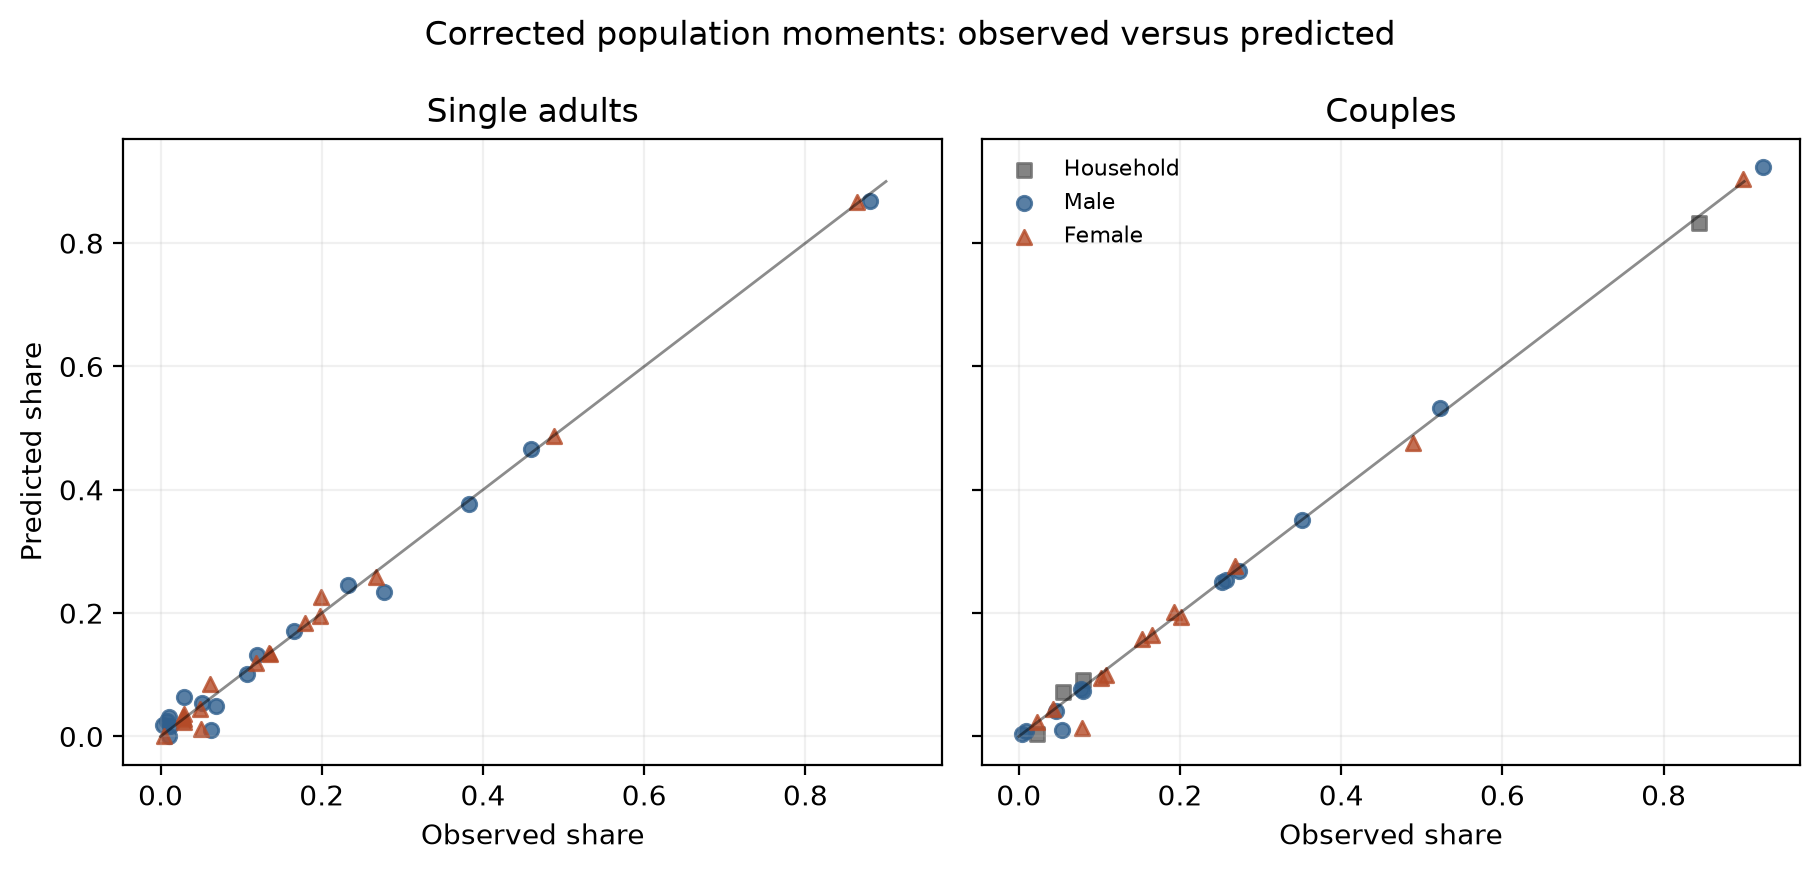
\includegraphics[height=0.72\textheight,width=\textwidth,keepaspectratio]{fit_by_margin_v7.png}
\end{center}
\backnav{main:est}
\note{Corrected population fit: observed against predicted shares, margin by
margin. Participation and occupation margins are reproduced closely in aggregate;
the hours fit is uneven. Population predictions integrate the model over
opportunities and taste shocks, so this is not an in-sample fitted choice.}
\end{frame}

\begin{frame}
\frametitle{Backup: the thirty-seven-hour point}
\hypertarget{b:hours37}{}
\vfill
\begin{columns}[T,onlytextwidth]
\column{0.23\textwidth}\centering
\textbf{single men}\\[0.3em]{\Large \VGapSingleMen} \\ {\footnotesize pp}
\column{0.23\textwidth}\centering
\textbf{single women}\\[0.3em]{\Large \VGapSingleWomen} \\ {\footnotesize pp}
\column{0.23\textwidth}\centering
\textbf{coupled men}\\[0.3em]{\Large \VGapCoupledMen} \\ {\footnotesize pp}
\column{0.23\textwidth}\centering
\textbf{coupled women}\\[0.3em]{\Large \VGapCoupledWomen} \\ {\footnotesize pp}
\end{columns}
\vfill
\begin{center}
{\small observed minus predicted share at the observed thirty-seven-hour mass point}
\end{center}
\vfill
\backnav{main:est}
\note{The common hours mismatch is underprediction of the observed concentration
at exactly thirty-seven hours. It is a finding about that mass point, not about
the model's neighbouring full-time range, and it is kept as its own result.}
\end{frame}

\begin{frame}
\frametitle{Backup: matched households}
\hypertarget{b:matched}{}
\begin{center}
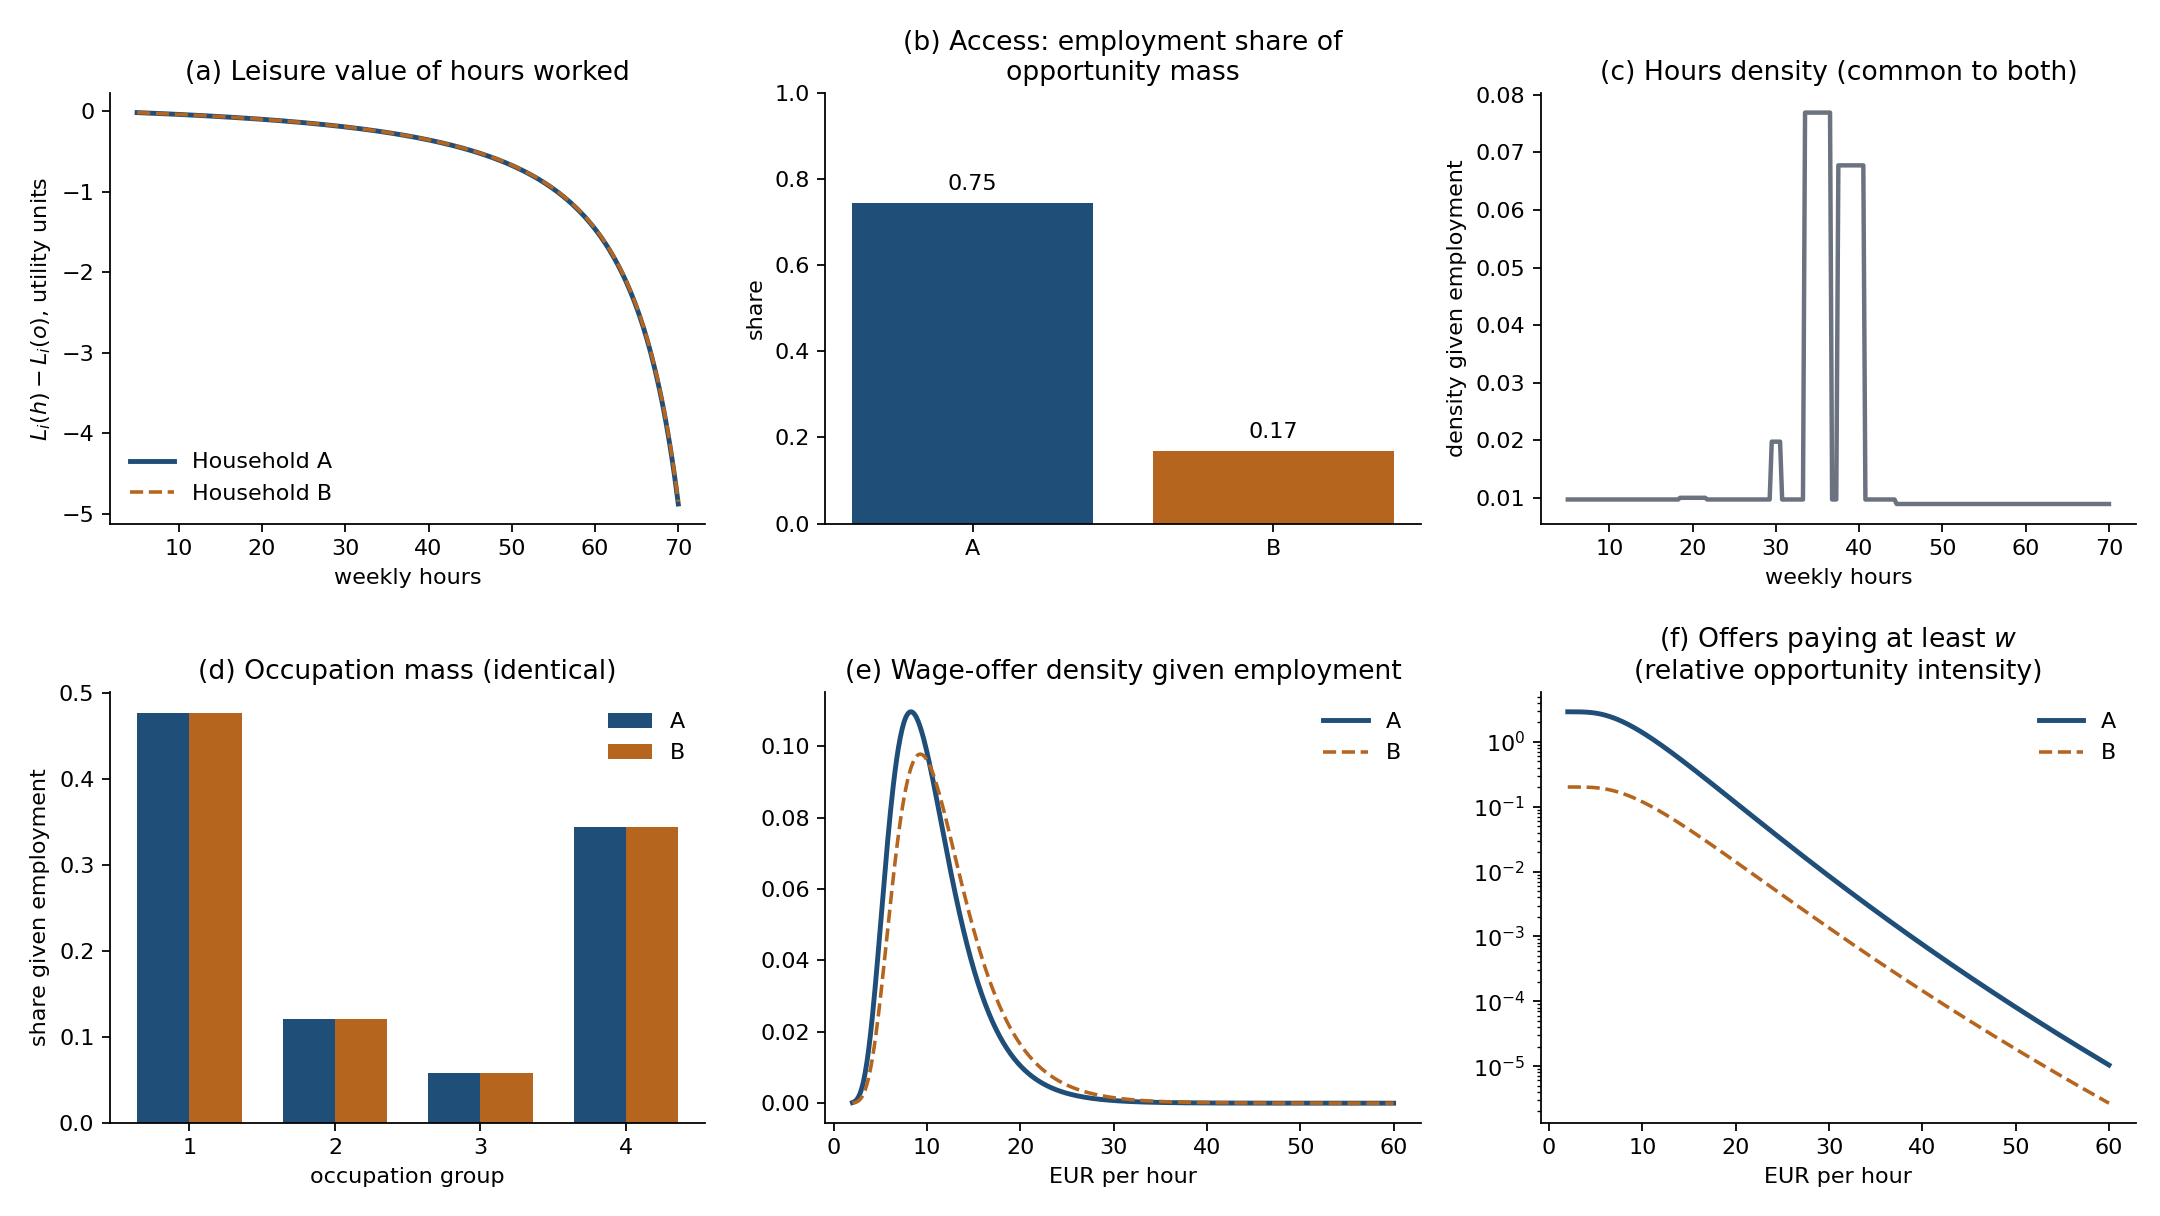
\includegraphics[height=0.64\textheight,width=\textwidth,keepaspectratio]{fig_matched_households_v11.png}
\end{center}
\begin{center}
{\footnotesize access: A $=$ \VMatchedAccessRatio{} $\times$ B \qquad wage-offer location: B $+$\VMatchedWageGap{} log points}
\end{center}
\backnav{main:opp}
\note{What unequal opportunity means inside the model. Two employed single men in
the same occupation group, hours band and wage quintile, with nearly identical
estimated leisure profiles, selected by a stated rule: a teaching example, not
causal and not representative. Employment is \VMatchedEmpShareA{} of A's
opportunity mass and \VMatchedEmpShareB{} of B's. B's wage offers are better, yet
A faces more offers paying at least any given wage over essentially all offer
mass. Neither is better placed on every margin.}
\end{frame}

\begin{frame}
\frametitle{Backup: marginal rate of substitution}
\hypertarget{b:mrs}{}
\begin{center}
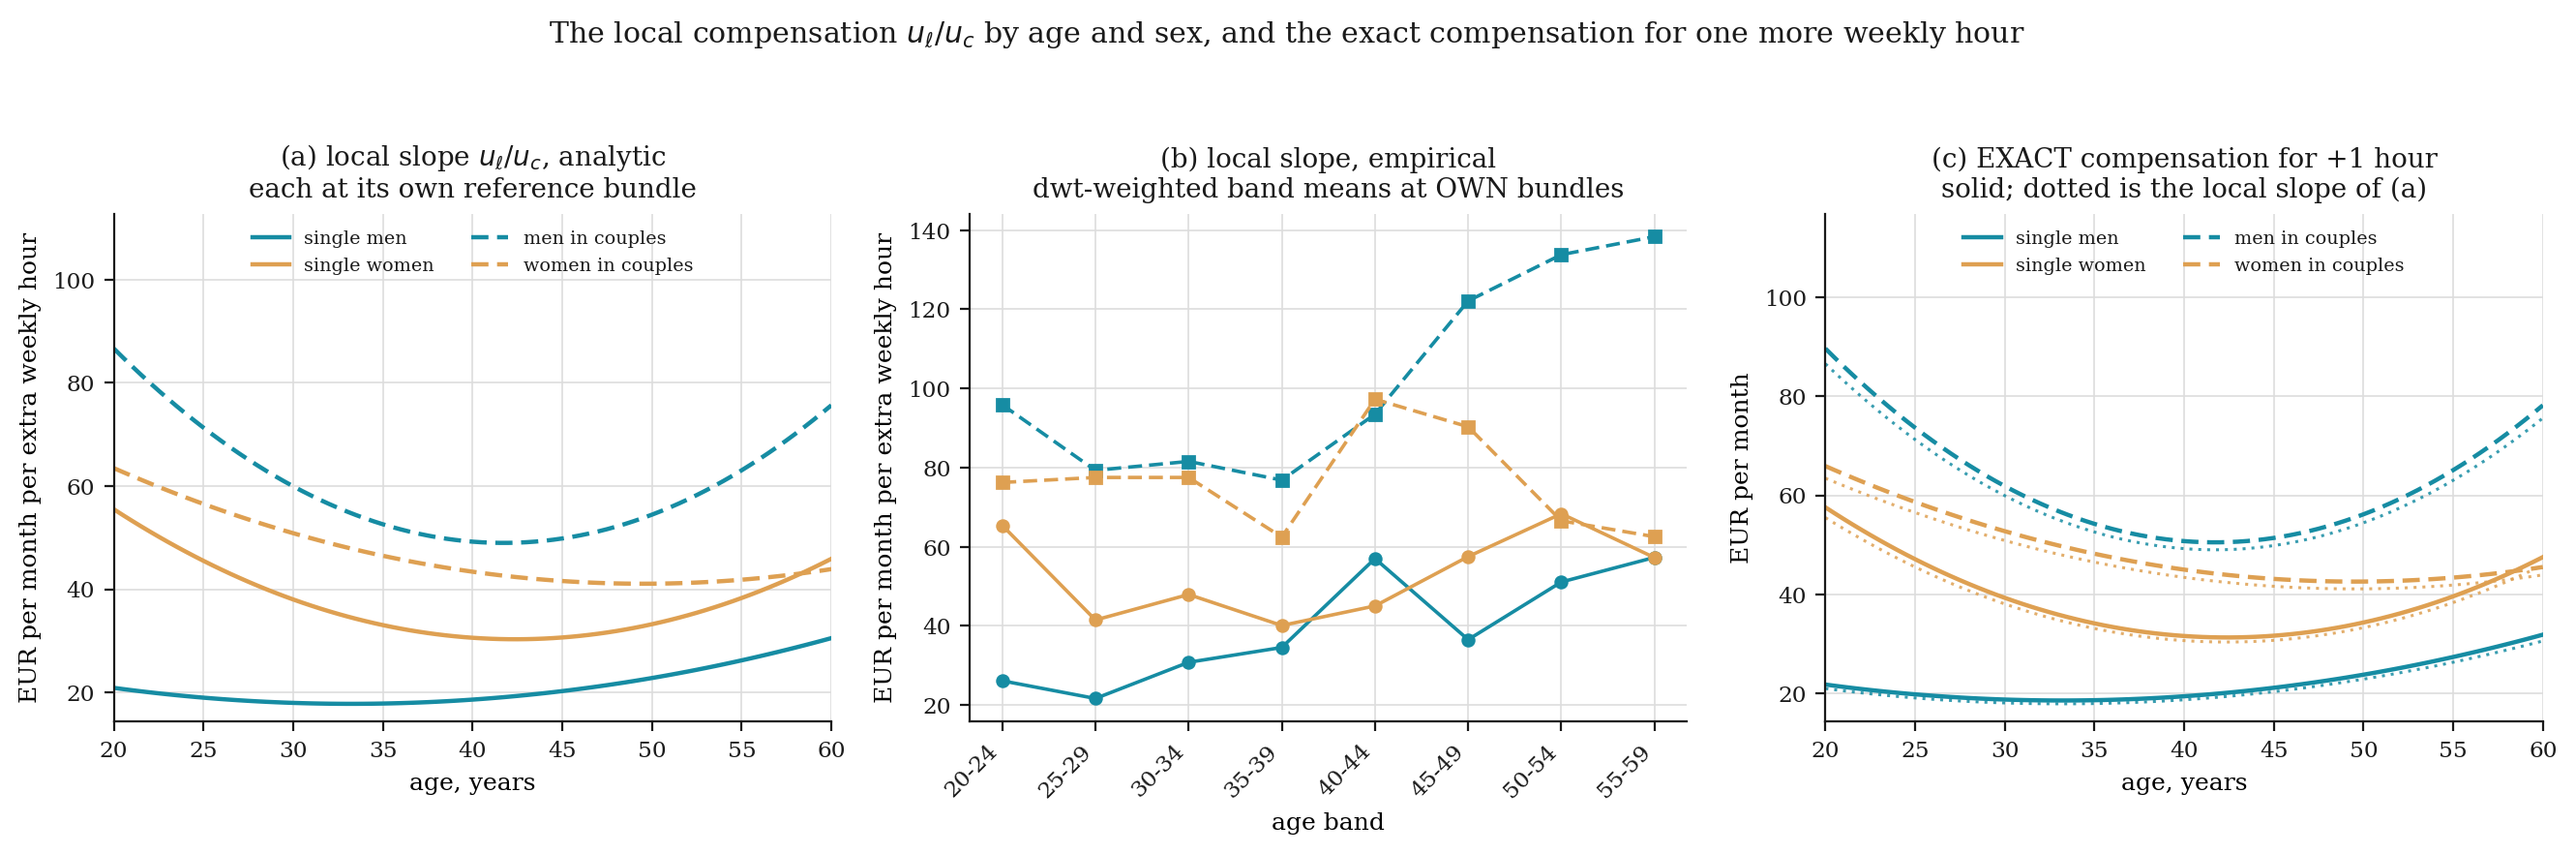
\includegraphics[height=0.72\textheight,width=\textwidth,keepaspectratio]{figP04_mrs_by_age_sex.png}
\end{center}
\backnav{main:sel}
\note{The marginal rate of substitution between leisure and consumption, by age
and sex, in euros per month per additional recurring weekly hour of leisure. It is
a compensation along an indifference curve, not a behavioural response to a wage
change. The coefficients are coordinates; this is the economics.}
\end{frame}

% ==================================================================== WELFARE
\begin{frame}
\frametitle{Backup: attained-bundle derivation}
\hypertarget{b:attderiv}{}
\vfill
\backupeq{$\displaystyle L_i(o)+\beta_c\log\!\Big(\frac{M^{\mathrm{att}}_i}{\lambda_c}\Big)=L_i(j^{\mathrm{obs}}_i)+\beta_c\log\!\Big(\frac{C^{\mathrm{obs}}_i}{\lambda_c}\Big)$}
\backupeq{$\displaystyle\Longrightarrow\quad M^{\mathrm{att}}_i=C^{\mathrm{obs}}_i\exp\!\Big\{\frac{L_i(j^{\mathrm{obs}}_i)-L_i(o)}{\beta_c}\Big\}$}
\vfill
\begin{columns}[T,onlytextwidth]
\column{0.46\textwidth}\centering
\textbf{Reference job}\\ {\footnotesize the preferred job when every job pays the same: here non-employment for every household}
\column{0.46\textwidth}\centering
\textbf{Staying-home equivalent}\\ {\footnotesize a verified property of this specification, not a general theorem}
\end{columns}
\vfill
\backnav{main:att}
\note{The attained-bundle money metric solves an indifference condition between
the observed job and consumption and the reference state at the unknown
consumption. The normaliser cancels. The general construction uses the job the
household would most prefer at equal pay; on the current domain non-employment
maximises the non-consumption index for every household, so the measure is the
staying-home equivalent. With a different leisure specification the two could
separate.}
\end{frame}

\begin{frame}
\frametitle{Backup: ex-ante derivation}
\hypertarget{b:eaderiv}{}
\vfill
\backupeq{$\displaystyle J_i=\int_{\Omega_i}e^{L_i(j)}\Big(\frac{C_i(j)}{\lambda_c}\Big)^{\beta_c}\widehat g_i(j)\,d\nu(j)$}
\backupeq{$\displaystyle J^{\mathrm{ref}}_i(m)=\Big(\frac{m}{\lambda_c}\Big)^{\beta_c}H_i,\qquad H_i=\int_{\Omega_i}e^{L_i(j)}\,\widehat g_i(j)\,d\nu(j)$}
\backupeq{$\displaystyle J^{\mathrm{ref}}_i\big(M^{\mathrm{EA}}_i\big)=J_i\quad\Longrightarrow\quad M^{\mathrm{EA}}_i=\lambda_c\exp\!\Big\{\frac{\log J_i-\log H_i}{\beta_c}\Big\}$}
\vfill
\begin{center}
{\small a common rescaling of $\widehat g_i$ cancels \quad$\cdot$\quad $\log J_i$: expected utility of the best reachable job, up to a constant}
\end{center}
\vfill
\backnav{main:ea}
\note{The reference prospect keeps the household's jobs, availability and
preferences and pays the same consumption at every job; its value is the power
of that consumption times H. Setting it equal to the actual prospect and solving
gives the ex-ante money metric. Under the extreme-value shocks, log J is the
expected utility of the best reachable job up to a constant common to J and H,
which is why taste-shock variety counts as welfare-relevant: a normative
position.}
\end{frame}

\begin{frame}
\frametitle{Backup: ex-ante numerical validation}
\hypertarget{b:eavalid}{}
\vfill
\begin{columns}[T,onlytextwidth]
\column{0.46\textwidth}
\centering
\textbf{Identities}\\[0.5em]
{\small constant-consumption identity}\\
{\small one-state identity}\\
{\small common intensity-rescaling invariance}\\
{\small flat-reference inversion}\\
{\small exact Shapley adding-up}
\column{0.46\textwidth}
\centering
\textbf{Numerics}\\[0.5em]
{\small exact reference integral on the priced set}\\
{\small effective sample size and weight concentration}\\
{\small two-seed stability of welfare, Gini and Shapley}\\
{\small finite positive welfare for every household}\\
{\small independent reimplementation}
\end{columns}
\vfill
\begin{center}
{\small all passed for both populations \quad$\cdot$\quad a correct computation, not causal identification or parameter uncertainty}
\end{center}
\vfill
\backnav{main:ea}
\note{The ex-ante calculation passed every declared check for both populations,
including an independent reimplementation, with the integration design fixed
before inspecting any welfare level or Shapley value. That certifies the
computation given the model and operators. It does not establish causal
identification, it does not quantify statistical uncertainty in the estimated
parameters, and it does not make either welfare perspective normatively correct.
Channel orderings are unchanged across the reported reference-domain
sensitivities.}
\end{frame}

\begin{frame}
\frametitle{Backup: equivalisation}
\hypertarget{b:equiv}{}
\vfill
\backupeq{$\displaystyle M^{p,\mathrm{eq}}_i=\frac{M^p_i}{e_i},\qquad e_i:\ \text{modified-OECD scale}$}
\vfill
\begin{columns}[T,onlytextwidth]
\column{0.46\textwidth}
\centering
\textbf{Couples, ex ante: A + B}\\[0.5em]
{\large \VEACoupOppRaw{}\% \quad$\longrightarrow$\quad \VEACoupOppEq{}\%}\\[0.3em]
{\footnotesize raw \quad$\to$\quad equivalised; \% of baseline Gini}
\column{0.46\textwidth}
\centering
\textbf{Couples, ex ante: preferences}\\[0.5em]
{\large \VEACoupPrefRaw{} \quad$\longrightarrow$\quad \VEACoupPrefEq{}}\\[0.3em]
{\footnotesize Gini points, raw \quad$\to$\quad equivalised}
\end{columns}
\vfill
\begin{center}
{\small a normative convention, reported both ways; populations never combined or compared}
\end{center}
\vfill
\backnav{main:howmuch}
\note{Equivalisation is a normative convention and it is consequential for couples
under the ex-ante perspective: it moves access plus earnings as a share of
baseline inequality and turns the preference contribution negative. A negative
Shapley term means that, averaged over orders, equalising preferences raises
inequality; it does not show that preference heterogeneity is equalising in any
causal or welfare sense. That is why both scales are always reported.}
\end{frame}

% ==================================================================== DECOMPOSITION
\begin{frame}
\frametitle{Backup: central figure}
\hypertarget{b:central}{}
\begin{center}
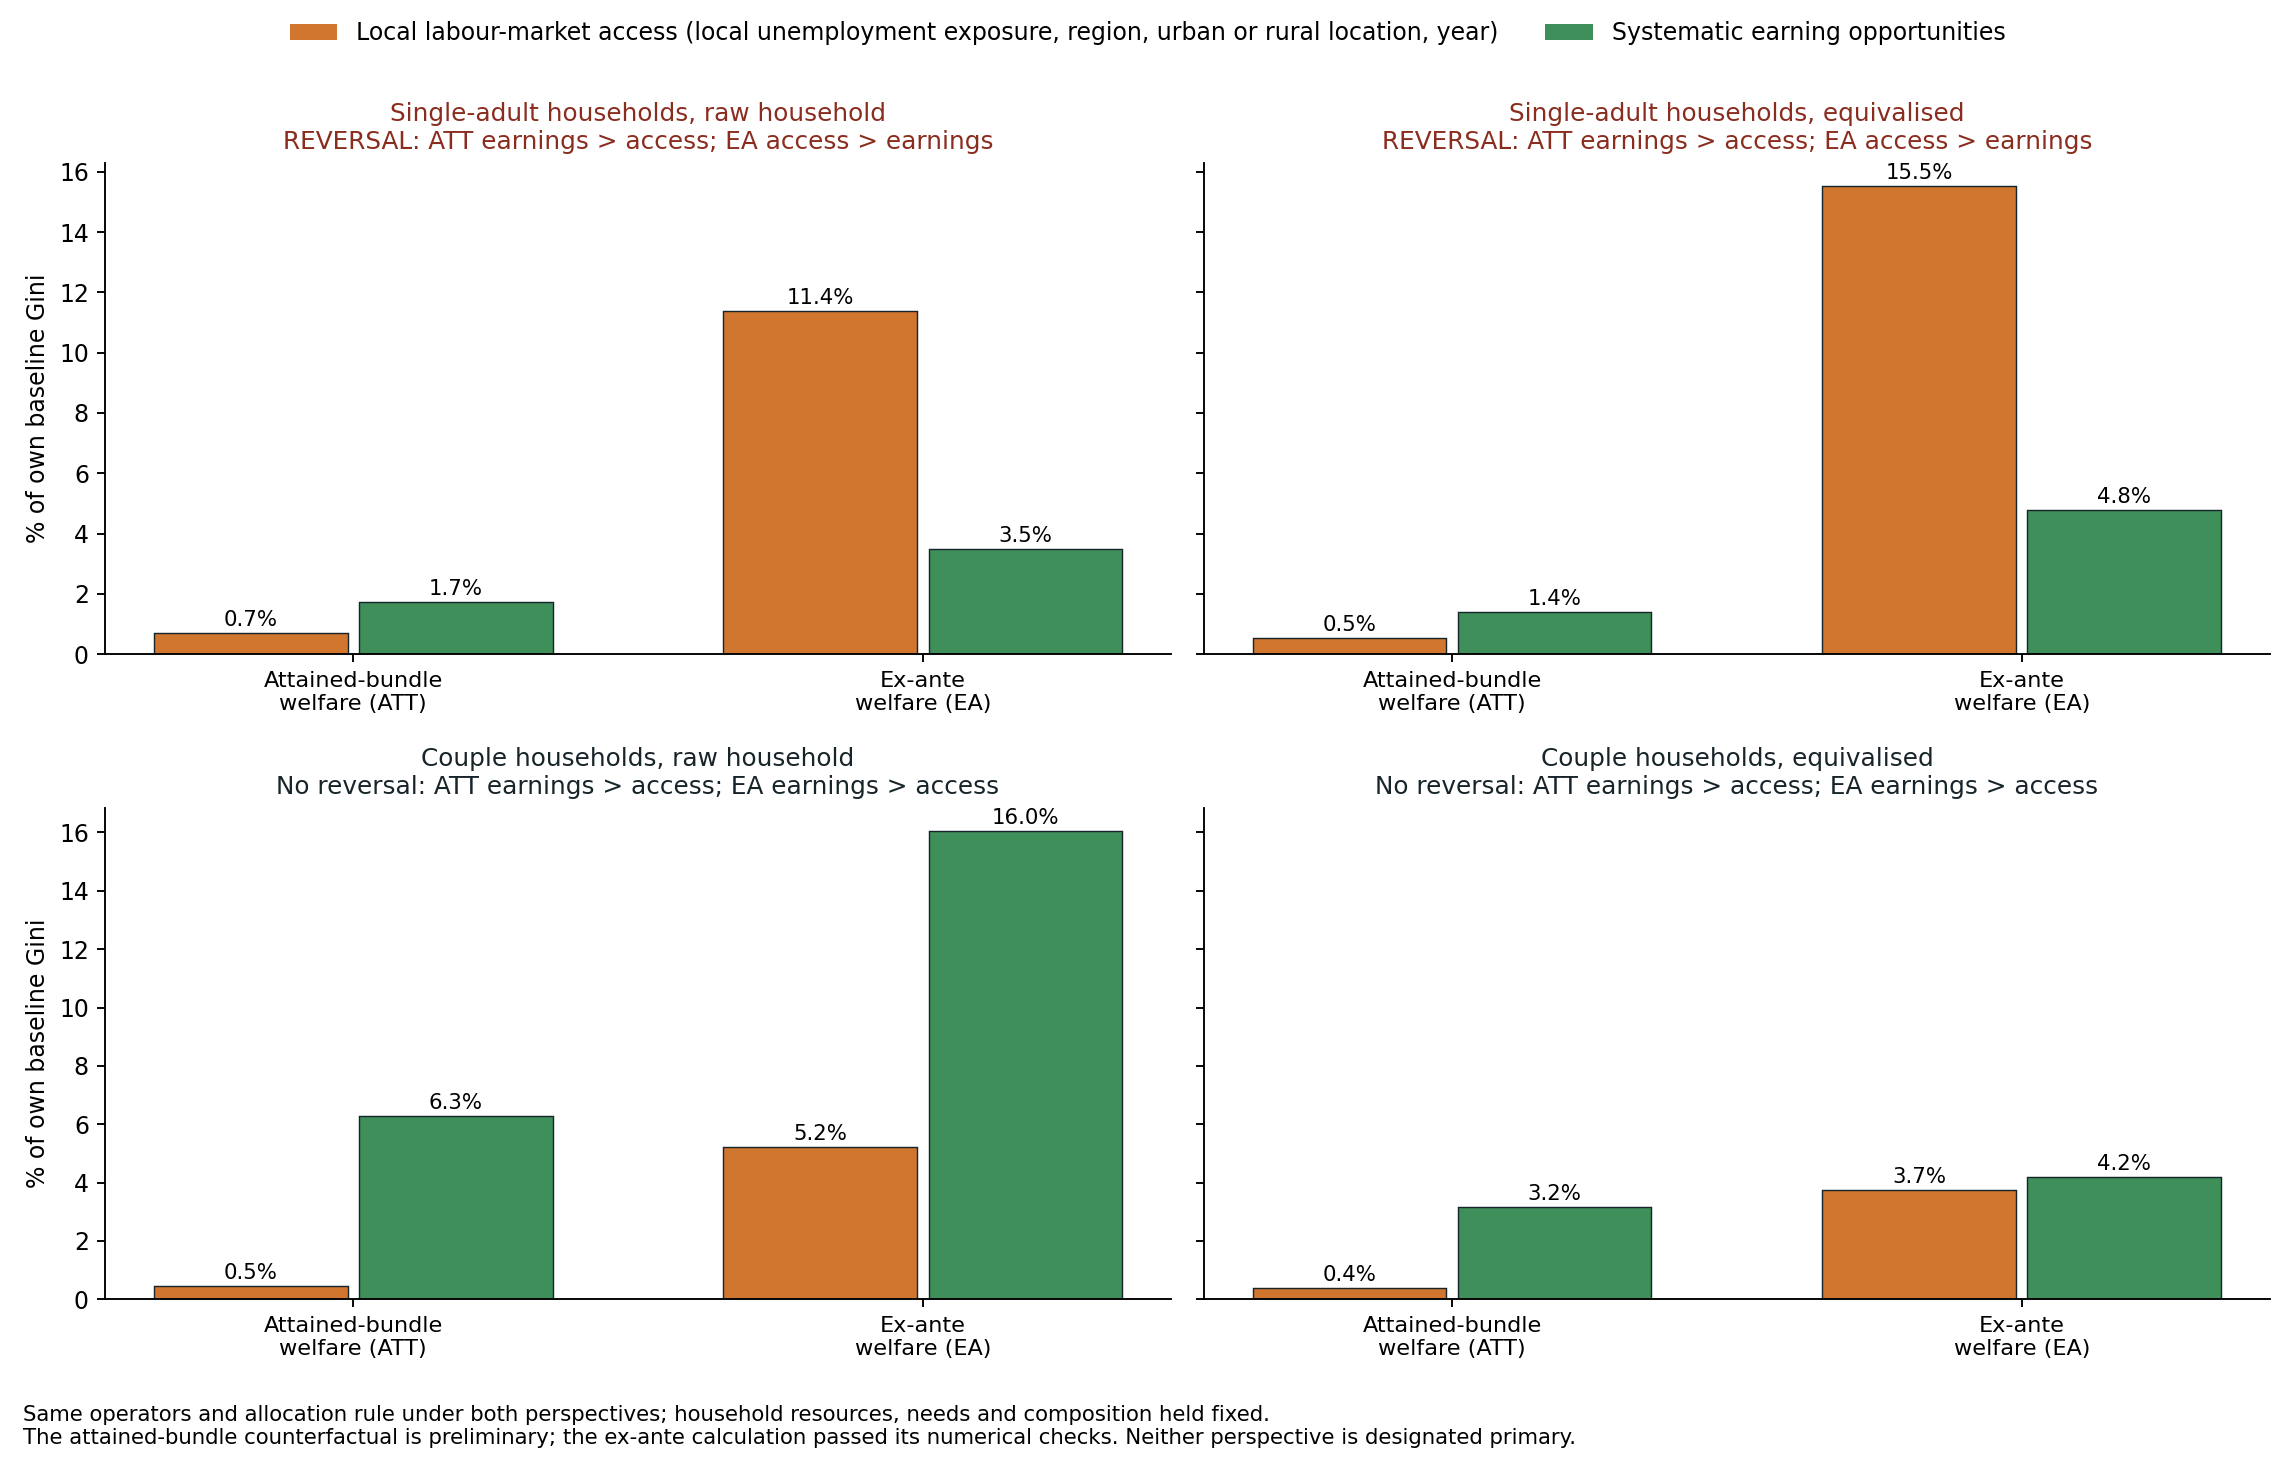
\includegraphics[height=0.72\textheight,width=\textwidth,keepaspectratio]{fig_v13_central_result.png}
\end{center}
\backnav{main:howmuch}
\note{The published central figure: access and earning-opportunity contributions,
each as a percentage of its own perspective's baseline Gini, under attained-bundle
and ex-ante welfare, raw and equivalised. For single adults earning
opportunities are larger under the attained bundle and access is larger under
the prospect; couples show no reversal. Resources, needs and composition are
held fixed.}
\end{frame}

\begin{frame}
\frametitle{Backup: ex-ante decomposition in Gini points}
\hypertarget{b:eagini}{}
\vfill
\begin{center}\scriptsize
\renewcommand{\arraystretch}{1.25}
\setlength{\tabcolsep}{4pt}
\begin{tabular}{llcccccl}
\toprule
 & scale & baseline Gini & \textcolor{chpref}{P} & \textcolor{chacc}{A} & \textcolor{chearn}{B} & A + B, \% of baseline & ordering \\
\midrule
Single adults & raw & \VEASingGiniRaw & \VEASingPhiPRaw & \VEASingPhiARaw & \VEASingPhiBRaw & \VEASingOppRaw & access $>$ earnings \\
 & equivalised & \VEASingGiniEq & \VEASingPhiPEq & \VEASingPhiAEq & \VEASingPhiBEq & \VEASingOppEq & access $>$ earnings \\
\midrule
Couples & raw & \VEACoupGiniRaw & \VEACoupPhiPRaw & \VEACoupPhiARaw & \VEACoupPhiBRaw & \VEACoupOppRaw & earnings $>$ access \\
 & equivalised & \VEACoupGiniEq & \VEACoupPhiPEq & \VEACoupPhiAEq & \VEACoupPhiBEq & \VEACoupOppEq & earnings $>$ access \\
\bottomrule
\end{tabular}
\end{center}
\vfill
{\footnotesize exact Shapley contributions in Gini points; household-weighted}
\backnav{main:howmuch}
\note{The full ex-ante table. Contributions are signed Gini points; access plus
earnings is reported relative to each baseline Gini. The calculation passed its
numerical checks, including an independent implementation. For couples the
preference contribution changes sign with equivalisation.}
\end{frame}

\begin{frame}
\frametitle{Backup: attained-bundle decomposition in Gini points}
\hypertarget{b:attgini}{}
\vfill
\begin{center}\scriptsize
\renewcommand{\arraystretch}{1.25}
\setlength{\tabcolsep}{4pt}
\begin{tabular}{llcccccl}
\toprule
 & scale & baseline Gini & \textcolor{chpref}{P} & \textcolor{chacc}{A} & \textcolor{chearn}{B} & A + B, \% of baseline & ordering \\
\midrule
Single adults & raw & \VAttFigSingGiniRaw & \VAttFigSingPhiPRaw & \VAttFigSingPhiARaw & \VAttFigSingPhiBRaw & \VAttSingOppRaw & earnings $>$ access \\
 & equivalised & \VAttFigSingGiniEq & \VAttFigSingPhiPEq & \VAttFigSingPhiAEq & \VAttFigSingPhiBEq & \VAttSingOppEq & earnings $>$ access \\
\midrule
Couples & raw & \VAttFigCoupGiniRaw & \VAttFigCoupPhiPRaw & \VAttFigCoupPhiARaw & \VAttFigCoupPhiBRaw & \VAttCoupOppRaw & earnings $>$ access \\
 & equivalised & \VAttFigCoupGiniEq & \VAttFigCoupPhiPEq & \VAttFigCoupPhiAEq & \VAttFigCoupPhiBEq & \VAttCoupOppEq & earnings $>$ access \\
\bottomrule
\end{tabular}
\end{center}
\vfill
{\footnotesize exact Shapley contributions in Gini points; preliminary; household-weighted}
\backnav{main:howmuch}
\note{The attained-bundle table. Earning opportunities are larger than local
access for both household types and both scales. The preference contribution
changes sign with equivalisation in both samples, so no directional claim is made
about it. The lower part of the hours range is sparsely represented in the
integration sample, which is why this exercise stays preliminary.}
\end{frame}

\begin{frame}
\frametitle{Backup: ex-ante channels, \% of baseline}
\hypertarget{b:eapct}{}
\vfill
\begin{center}\footnotesize
\renewcommand{\arraystretch}{1.3}
\setlength{\tabcolsep}{4pt}
\begin{tabular}{llc cc cc cc}
\toprule
 & & & \multicolumn{2}{c}{\textcolor{chpref}{P}} & \multicolumn{2}{c}{\textcolor{chacc}{A}} & \multicolumn{2}{c}{\textcolor{chearn}{B}} \\
 & scale & $I_0$ & Gini pts & \% of $I_0$ & Gini pts & \% of $I_0$ & Gini pts & \% of $I_0$ \\
\midrule
Single adults & raw & \VEASingGiniRaw & \VEASingPhiPRaw & \VPctEASingPRaw & \VEASingPhiARaw & \VPctEASingARaw & \VEASingPhiBRaw & \VPctEASingBRaw \\
 & equivalised & \VEASingGiniEq & \VEASingPhiPEq & \VPctEASingPEq & \VEASingPhiAEq & \VPctEASingAEq & \VEASingPhiBEq & \VPctEASingBEq \\
\midrule
Couples & raw & \VEACoupGiniRaw & \VEACoupPhiPRaw & \VPctEACoupPRaw & \VEACoupPhiARaw & \VPctEACoupARaw & \VEACoupPhiBRaw & \VPctEACoupBRaw \\
 & equivalised & \VEACoupGiniEq & \VEACoupPhiPEq & \VPctEACoupPEq & \VEACoupPhiAEq & \VPctEACoupAEq & \VEACoupPhiBEq & \VPctEACoupBEq \\
\bottomrule
\end{tabular}
\end{center}
\vfill
{\footnotesize each contribution divided by its own baseline Gini $I_0$; signed; the rows are not forced to sum to one hundred, because the remainder is not allocated by this exercise}
\cornerlinks{\hyperlink{main:channel}{\beamerreturnbutton{Back}}\ \hyperlink{appmap}{\beamergotobutton{Appendix map}}\ \golink{b:explained}{composition within P/A/B}}
\note{Each ex-ante Shapley contribution, in Gini points and as a percentage of its
own baseline Gini, raw and equivalised. The negative couples preference term is
kept. P, A and B do not exhaust baseline inequality: household resources, needs
and composition and other dimensions are held fixed or left unallocated.}
\end{frame}

\begin{frame}
\frametitle{Backup: attained-bundle channels, \% of baseline}
\hypertarget{b:attpct}{}
\vfill
\begin{center}\footnotesize
\renewcommand{\arraystretch}{1.3}
\setlength{\tabcolsep}{4pt}
\begin{tabular}{llc cc cc cc}
\toprule
 & & & \multicolumn{2}{c}{\textcolor{chpref}{P}} & \multicolumn{2}{c}{\textcolor{chacc}{A}} & \multicolumn{2}{c}{\textcolor{chearn}{B}} \\
 & scale & $I_0$ & Gini pts & \% of $I_0$ & Gini pts & \% of $I_0$ & Gini pts & \% of $I_0$ \\
\midrule
Single adults & raw & \VAttFigSingGiniRaw & \VAttFigSingPhiPRaw & \VPctAttSingPRaw & \VAttFigSingPhiARaw & \VPctAttSingARaw & \VAttFigSingPhiBRaw & \VPctAttSingBRaw \\
 & equivalised & \VAttFigSingGiniEq & \VAttFigSingPhiPEq & \VPctAttSingPEq & \VAttFigSingPhiAEq & \VPctAttSingAEq & \VAttFigSingPhiBEq & \VPctAttSingBEq \\
\midrule
Couples & raw & \VAttFigCoupGiniRaw & \VAttFigCoupPhiPRaw & \VPctAttCoupPRaw & \VAttFigCoupPhiARaw & \VPctAttCoupARaw & \VAttFigCoupPhiBRaw & \VPctAttCoupBRaw \\
 & equivalised & \VAttFigCoupGiniEq & \VAttFigCoupPhiPEq & \VPctAttCoupPEq & \VAttFigCoupPhiAEq & \VPctAttCoupAEq & \VAttFigCoupPhiBEq & \VPctAttCoupBEq \\
\bottomrule
\end{tabular}
\end{center}
\vfill
{\footnotesize each contribution divided by its own baseline Gini $I_0$; signed; preliminary}
\backnav{main:channel}
\note{The same layout for the attained-bundle perspective. Earning opportunities
exceed access in every row; the preference contribution changes sign with
equivalisation. These percentages are shares of each baseline Gini and are not
forced to sum to one hundred.}
\end{frame}

\begin{frame}
\frametitle{Backup: composition of the explained component}
\hypertarget{b:explained}{}
\vfill
\backupeq{$\displaystyle s_k=\frac{\phi_k}{\phi_P+\phi_A+\phi_B},\qquad k\in\{P,A,B\}$}
\vfill
\begin{center}\small
\renewcommand{\arraystretch}{1.35}
\begin{tabular}{lrr}
\toprule
ex-ante prospect, equivalised & Single adults & Couples \\
\midrule
\textcolor{chpref}{Preferences} $s_P$ & \VExplSingP\% & \VExplCoupP\% \\
\textcolor{chacc}{Local access} $s_A$ & \VExplSingA\% & \VExplCoupA\% \\
\textcolor{chearn}{Earning opportunities} $s_B$ & \VExplSingB\% & \VExplCoupB\% \\
\midrule
Total & \VExplSingTotal\% & \VExplCoupTotal\% \\
\bottomrule
\end{tabular}
\end{center}
\vfill
{\footnotesize These are shares of the currently explained P/A/B change, not shares of total inequality. Negative components are possible under Shapley attribution.\par}
\backnav{b:eapct}
\note{These are shares of the currently explained P/A/B change, not shares of
total inequality. Negative components are possible under Shapley attribution.

Within that currently explained component, most of the single-adult opportunity
effect comes through access rather than earning opportunities. For couples the
negative preference share means the access and earning shares together exceed
the whole explained change. Only the equivalised scale is shown: on the raw scale
the one-decimal couples shares would not close exactly.}
\end{frame}

\begin{frame}
\frametitle{Backup: Shapley versus one-factor equalisation}
\hypertarget{b:shapley}{}
\vfill
\backupeq{$\displaystyle \text{one-factor:}\quad v^p(\{k\})=I^p(\varnothing)-I^p(\{k\})$}
\backupeq{$\displaystyle \text{Shapley:}\quad \phi^p_k=\text{average over all orders of } v^p(S\cup\{k\})-v^p(S)$}
\backupeq{$\displaystyle \phi^p_P+\phi^p_A+\phi^p_B=I^p(\varnothing)-I^p(\{P,A,B\})$}
\vfill
\begin{center}
{\small one-factor effects need not add up \quad$\cdot$\quad Shapley contributions do, exactly}
\end{center}
\vfill
\backnav{main:shapley}
\note{A one-factor effect equalises one channel from the actual situation. Because
the channels interact, those effects need not add up, and the answer would depend
on the order chosen. The Shapley contribution averages each channel's marginal
effect over every order and adds up exactly to the total change. This is the
standard rule from the distributional decomposition literature; no new principle
is claimed. Coalition-by-coalition Gini tables are not reproduced in these
slides.}
\end{frame}

\begin{frame}
\frametitle{Backup: what is not allocated}
\hypertarget{b:residual}{}
\vfill
\begin{columns}[T,onlytextwidth]
\column{0.31\textwidth}\centering
\textbf{Held fixed}\\[0.4em]
{\footnotesize household resources, needs and composition}
\column{0.31\textwidth}\centering
\textbf{Retained}\\[0.4em]
{\footnotesize sex- and household-type-specific preference and opportunity blocks}
\column{0.31\textwidth}\centering
\textbf{Not equalised}\\[0.4em]
{\footnotesize wage-draw luck and the common offer spread}
\end{columns}
\vfill
\begin{center}
wage-offer location differences: at most about \VOfferLocation{} log points\\[0.3em]
common offer spread: about \VOfferSpread{} log points
\end{center}
\vfill
\begin{center}
{\small next: household resources, needs and composition as a fourth channel D; A + B stays the opportunity component}
\end{center}
\backnav{main:hundred}
\note{The not-allocated remainder is not a channel. It holds household resources,
needs and composition fixed, it keeps the sex- and household-type-specific
blocks, and it excludes wage-draw luck and the common offer spread. The location
differences that the earning operator equalises are small next to that common
spread, so the operator removes only a small part of earnings dispersion by
construction; that is a definitional boundary, not a measurement error. Adding a
fourth channel for resources, needs and composition is the planned extension;
with it, access plus earnings would still be the opportunity component, and the
broader sum would not be an opportunity share.}
\end{frame}

\begin{frame}
\frametitle{Backup: robustness of the attained-bundle decomposition}
\hypertarget{b:robust}{}
\vfill
\begin{columns}[T,onlytextwidth]
\column{0.46\textwidth}
\centering
\textbf{Second simulation seed}\\[0.5em]
{\small every coalition Gini and contribution reproduces closely, including the preference sign change}
\column{0.46\textwidth}
\centering
\textbf{Observed job in the simulation}\\[0.5em]
{\small attained under every coalition by \VObsJobShareSingles\% of single adults and \VObsJobShareCouples\% of couples}\\[0.3em]
{\small excluding it moves the total change by at most \VObsJobMove\%, with no sign change}
\end{columns}
\vfill
\begin{center}
{\small simulation checks, not confidence intervals}
\end{center}
\vfill
\backnav{main:limits}
\note{Robustness of the attained-bundle calculation. An independent second seed
reproduces every coalition Gini and Shapley contribution closely. The simulation
always includes each household's own observed job; excluding it moves the total
change by at most the amount shown, in the couples equivalised case, with no sign
change. These checks validate the calculation for the stated game, not its
maintained assumptions, and they are not confidence intervals.}
\end{frame}

% ==================================================================== DATA
\begin{frame}
\frametitle{Backup: sample selection}
\hypertarget{b:sample}{}
\vfill
\begin{center}\scriptsize
\renewcommand{\arraystretch}{1.15}
\begin{tabular}{>{\raggedright\arraybackslash}p{0.56\textwidth}rr}
\toprule
screen & single-adult & couple \\
\midrule
\VFunnelZeroLabel & \VFunnelZeroSingles & \VFunnelZeroCouples \\
\VFunnelOneLabel & \VFunnelOneSingles & \VFunnelOneCouples \\
\VFunnelTwoLabel & \VFunnelTwoSingles & \VFunnelTwoCouples \\
\VFunnelThreeLabel & \VFunnelThreeSingles & \VFunnelThreeCouples \\
\VFunnelFourLabel & \VFunnelFourSingles & \VFunnelFourCouples \\
\VFunnelFiveLabel & \VFunnelFiveSingles & \VFunnelFiveCouples \\
\VFunnelSixLabel & \VFunnelSixSingles & \VFunnelSixCouples \\
\VFunnelSevenLabel & \VFunnelSevenSingles & \VFunnelSevenCouples \\
\VFunnelEightLabel & \VFunnelEightSingles & \VFunnelEightCouples \\
\VFunnelNineLabel & \VFunnelNineSingles & \VFunnelNineCouples \\
\midrule
\textbf{estimation sample} & \textbf{\VNSingles} & \textbf{\VNCouples} \\
\bottomrule
\end{tabular}
\end{center}
\vfill
\backnav{main:data}
\note{Unweighted households remaining after each screen. The largest exclusion is
structural: multi-generational households, flat-shares and same-sex couples are
outside the estimated population, and no result extends to them. Students and
pension recipients are removed because the model does not define an offer set for
them; the remaining screens are support restrictions.}
\end{frame}

\begin{frame}
\frametitle{Backup: EUROMOD pricing}
\hypertarget{b:pricing}{}
\vfill
\begin{columns}[T,onlytextwidth]
\column{0.31\textwidth}\centering
\textbf{Inputs}\\[0.4em]
{\footnotesize a work arrangement: hours, hourly wage, earnings split; household roster and non-labour inputs}
\column{0.31\textwidth}\centering
\textbf{EUROMOD}\\[0.4em]
{\footnotesize French \VPolicyYear{} policy system; only deciders receive counterfactual overrides}
\column{0.31\textwidth}\centering
\textbf{Output}\\[0.4em]
{\footnotesize $C_i(j)$: household disposable income, summed over all members}
\end{columns}
\vfill
\begin{center}
{\small every sampled alternative and every welfare integration point is priced}\\[0.3em]
{\small tax-benefit accounting identity holds to machine precision}
\end{center}
\vfill
\backnav{main:data}
\note{For a given work arrangement the tax-benefit model receives the implied
gross labour inputs together with the household's non-labour inputs and roster,
and returns disposable income. Only deciders receive counterfactual overrides;
other members keep their baseline values. The accounting identity linking
original income, benefits, taxes and contributions to disposable income holds to
machine precision at the person and household-alternative level.}
\end{frame}

\begin{frame}
\frametitle{Backup: numerical design}
\hypertarget{b:numerics}{}
\vfill
\begin{columns}[T,onlytextwidth]
\column{0.31\textwidth}\centering
\textbf{Estimation}\\[0.4em]
{\Large \VNAltRows}\\ {\footnotesize rows per household: the observed job and \VNDraws{} sampled alternatives}
\column{0.31\textwidth}\centering
\textbf{Predictive fit}\\[0.4em]
{\Large \VNNodes}\\ {\footnotesize common integration points per household}
\column{0.31\textwidth}\centering
\textbf{Supports}\\[0.4em]
{\Large $[\VHoursFloor,\VHoursCap]$}\\ {\footnotesize weekly hours; wages in $[\VWageLo,\VWageHi]$ per hour}
\end{columns}
\vfill
\begin{center}
{\small sampling devices are computational: they are not offers and enter no welfare measure}
\end{center}
\vfill
\backnav{main:data}
\note{The numerical design. Estimation uses the observed job plus sampled
alternatives per household. The predictive fit integrates over a separate, larger
common set of priced integration points per household. The supports are the
intervals on which the opportunity densities are defined. The ex-ante welfare
integrals use their own certified design, chosen before any welfare result was
inspected.}
\end{frame}

\end{document}
